\chapter{Artificial Neural Networks for EHL Film Thickness Predictions}
\label{ANN Lubricated Bearing FMBD}

\section{Abstract}

Tribodynamic modelling generally employs analytical equations for the prediction of film thickness in elastohydrodynamic contacts; chosen due to their timely solution. Whilst computationally efficient, these do not achieve the accuracy of the full numerical solution outside the bounds of the data used to generate the analytical equations. In the context of dynamic simulation, a full numerical solution at each time step of a system level model would, however, yield excessive computation time. This has led to the emerging use of data driven solutions, such as machine learning, in the field of tribology. These can achieve accuracy much closer to the numerical solution, whilst significantly improving computational time.

This chapter details the development of an ANN for prediction of central film thickness at the roller-race conjunction. ANNs are trained using data generated by numerical solution, with the data set constrained to realistic operating conditions using the Greenwood regimes of lubrication. Multiple ANNs are compared to find the optimum structure, accounting for training time and accuracy.

This workflow introduces the application of Artificial Neural Networks (ANNs) a form of Machine Learning (ML) algorithm, to predict the central film thickness at the roller-race conjunction. The performance of ANNs will be compared with analytical equations and numerical solutions, assessing the suitability of its implicit application within FMBD environments. The aim is to improve the accuracy of the central film thickness estimation, whilst maintaining a timely solution in the context of a full dynamic solution.



\section{Introduction}


Two main approaches exist for determination of the complex non-linear problem of film thickness in lubricated contacts. The first approach involves employing numerical methods \cite{Dowson1959}, where systems of partial differential equations are formulated to describe the state of the contact and then solved iteratively \cite{Gohar2018}. While this method yields accurate results and is applicable to a wide range of operating conditions, it is computationally intensive due to its iterative nature. The second approach involves developing regressed analytical equations from experimental or numerical studies which can be used for specific lubrication regimes. These equations offer quick estimates of key parameters, such as central \cite{Dowson1979} and minimum film thickness \cite{Dowson1967}. However, whilst more computationally efficient than full numerical solutions, this approach has limitations. The applicability of regressed equations is often limited to the range of data used for their development, resulting in reduced accuracy due to simplification. There is also a requirement for extensive effort in collecting experimental or numerical data to develop them. The implementation of ANNs within tribology is one  Although ANNs lack the physical understanding provided by numerical solutions, they offer nearly real-time performance comparable to analytical solutions while benefiting from the accuracy of numerical methods \cite{EchavarriOtero2014}. To ensure the validity of the ANN, a methodology is suggested for training it within a range consistent with the numerical solver.

The most common ML algorithm used in tribological applications are ANNs. The first utilization of these were in the 1990s \cite{Argatov2019}. Ezugwu et al. implemented and ANN for wear rate and hence life predictions of ceramic cutting tools \cite{Ezugwu1995}. Their model had an 80\% success rate in predicting the failure mechanism of the tools. Rutherford et al. \cite{Rutherford1996} and Jones et al. \cite{Jones1997} developed on this success, focussing on wear rate predictions for coating materials and mechanical systems respectively. Jones et al. were able to achieve 90\% wear rate predication accuracy by optimising their ANN architecture using $R^2$ coefficients as a performance indicator. Similar studies were then conducted in the domain of friction and wear rate of composite materials \cite{Genel2003} \cite{Hayajneh2009} \cite{Zhang2002}, as well as tools steels \cite{Cavaleri2019}. 

Whilst the friction in the aforementioned studies was modelled under dry conditions, friction in lubricated contacts has also been modelled using ANNs. Bhaumik et al. \cite{Bhaumik2019a} used ANNs to develop a new lubricant with multiple friction modifiers (FM), considering load, speed and FM concentration as input variables, with the target output being coefficient of friction. A similar methodology was employed to develop biodegradable oils \cite{Bhaumik2019a}, validating both sets of studies using pin-on-disc friction measurements. Traction coefficients under various thermal-elastohydrodynamic operating conditions have also been investigated \cite{EchavarriOtero2014}, with the authors noting fast predictions of results with excellent accuracy (lower than 3\% error in most cases). Further lubricated studies involving relative viscosity predictions \cite{Afrand2016} \cite{HemmatEsfe2018} have achieved deviation margins of 1.5\% and 0.07\% respectively, substantially lower than empirical correlations.

Many further studies have been performed in the field of wear in manufacturing processes \cite{Ripa2004}. Previous studies had multiple input variables to the ANNs (speed, load, temperature, shear rate). For specific manufacturing processes with particular lubricant-surface combinations, the input data array can be drastically reduced to process-specific variables such as load, speed, and vibration. This approach was taken to investigate flank wear in drilling \cite{Panda2008} and surface roughness of machined parts \cite{Asilturk2011}. By reducing the number of input parameters, less training data was required to achieve good fits.

The studies referenced (\cite{Ezugwu1995} - \cite{Asilturk2011}) all shared a common approach of utilizing experimental data to train the ANNs. Whilst experimental data benefits from the lack of assumptions in numerical models, there is the limitation of high costs and time required for generating large datasets. Consequently, the training datasets for the ANN were limited to approximately one hundred points \cite{Zhang2002} \cite{Hayajneh2009}, or fewer \cite{Ezugwu1995} \cite{Rutherford1996}, with the largest (216 points) utilised by Cavaleri et al. \cite{Cavaleri2019}. Since the training process optimizes the ability of the ANN to interpolate between data points for varying input conditions, a greater number of training points is advantageous. It was noted by Ezugwu et al. \cite{Ezugwu1995} and Zhang et al. \cite{Zhang2002} that a significant improvement in ANN fit was achieved with a larger training data set. This is an observation shared across several studies and scientific applications \cite{Barbedo2018}.

An alternative method of achieving large data sets without the high financial and time cost of experimentation is to use numerical modelling. Wang et al. \cite{Wang2020} identified the need for larger training sets in the field of tribology. Their prediction for maximum Hertzian pressure in thermohydrodynamic contacts utilised a training data set that was generated using Reynolds equation. Whilst limited to the accuracy of the numerical model, the ANN benefits from much faster computation time. It crucially also allows for larger data sets to be generated that can cover a much larger range of input data; a requirement for implementation within dynamic models.

The Reynolds boundary value problem has also been solved using Physics Informed Neural Networks (PINN) by Almqvist \cite{Almqvist2021}. The study was not to improve on the numerical accuracy or efficiency of standard finite-difference based methods, rather to present an application of PINN in the field of tribology. Error analysis showed good agreement with the analytical solution, however further work is needed to improve the solving efficiency. Since the ANN is to be implicitly embedded within a dynamic simulation, efficiency is critical. Data driven solutions are therefore preferable. Marian et al. \cite{Marian2022} demonstrated for the first time the generation of EHL film thickness data using a Finite Element Method (FEM) to train an ANN. The ANNs could predict locally-resolved film thickness across the contact domain 25-times faster than FE-based EHL simulations.


It is now known that data-driven solutions, such as machine learning, can greatly enhance the computational efficiency of tribo-dynamic simulations without sacrificing accuracy. In this study, artificial neural networks (ANNs) were trained using numerical solutions constrained by lubrication regimes to ensure the quality of the training data set.


\section{Artificial Neural Network Fundamentals}

Artificial intelligence (AI) refers to machines that exhibit human cognitive skills. They are a set of algorithms which allow machines to learn and problem solve in a manner inspired by the neurons in the human brain. Machine learning (ML), a subset of AI, allow systems to perform tasks without explicit programming. These algorithms analyse data and autonomously adapt to enhance their task performance, resembling the human ability to learn from experience. 

ML encompasses two primary algorithm types: supervised learning and unsupervised learning. In supervised learning, the program receives both input data and target outputs. The programmer guides the algorithm by demonstrating the correct output. The program can then compare its own outputs to the desired ones, refining itself through training. For example, by training on images and corresponding object names, the program can subsequently recognize objects in new images unassisted. Unsupervised learning algorithms operate without target outputs, exploring input data for patterns independently. These algorithms analyse the input's feature space and cluster the data accordingly. When presented with new data, the program assigns it to an existing cluster based on its location in the feature space.

ML algorithms can also be classified based on the type of output they produce. They can be utilized for classification problems, where data points are assigned to discrete categories, or regression problems, involving approximating continuous output functions. Classification tasks can be accomplished through supervised learning algorithms using logistic regression, approximating step functions with discrete outputs. Unsupervised learning algorithms achieve classification through clustering, an example of which being character recognition and speech processing,image and speech processing.

Supervised ML algorithms have the advantage of approximating continuous output functions, making them suitable for complex nonlinear relationships between inputs and outputs. By comparing their outputs with target values during training, they act as universal function approximators. This characteristic proves particularly valuable for applications such as tribological simulation, where the interaction between contacting surfaces requires efficient solvers. Notably, supervised linear regression ML algorithms offer effective solutions in this domain.









\subsection{Numerical EHL Methodology}

\subsection{Artificial Neural Network Methodology}

An Artifical Neural Network (ANN) is a computational model which is inspired by the neural networks present in the human brain. It is a subset of machine learning.

ANNs are made up of a set of interconnected nodes that have the ability to adapt to input data for the purpose of solving complex non-linear functions. The nodes, known as artificial neurons, are organized into layers. The three main types of layers are shown in FIGURE 1, these are: Input layer; Hidden layer(s) and Output layer. The adaptation is performed using weighted connections, that connect each neuron layer. These weightings can be adapted during the learning process, and determine the strength of the connections between neurons.

The generalized structure of an ANN comprises several layers which contain neurons inside. Equation \ref{Generalized ANN} describes the relationship between each neuron, $i$, of each layer, $j$,

\begin{equation}\label{Generalized ANN}
	u_i^{j, k}=f_j\left(\sum_{\forall m} W_i^{j, k} \cdot x_m+b_i^{j, k}\right)
\end{equation}

\subsection{ANN Training Process}









The learning proccess of an ANN involves training a set of input data which correspond to known output values. A common technique for this is back propagation, where the connection weightings in the network are adjusted such that the error between the predicted and the actual output are minimized. The goal of this training is to minimize the error, and to improve the ability of the network to generalize and make accurate predictions for new, unseen data.

As the structural complexity of ANNs increases, the training time increases due to the greater number of neurons and layers. Implementations of ANN in the field of tribology, specifically film thickness predictions, are typically limited to between one and three hidden layers \cite{Marian2021}. 

MATLAB 2022a was used for the development of the ANNs.

The training data set for the ANN was obtained from numerical models. This decision was made due to the size of the database required for training, and the timely and relatively low resource-intensive nature to generate this. It is worth noting that training data could also be obtained from experimental work, which further enhances the applicability of this approach for future studies.

The structure of the ANN is described in the following format, as per \cite{Zhang2002}:

\begin{equation}
	N_{i n}-\left[N_{h 1}-N_{h 2}-N_{h 3}\right]_t-N_{\text {out }}
\end{equation}

The number of neurons in each layer is denote4d by the symbol $N$, with the input and output layers indicated by the subscripts $in$ and $out$, respectively. Subscripts $h1$, $h2$, and $h3$ denote the hidden layers, with $t$ being the total number of hidden layers.

To evaluate the performance of different ANN structures, a sensitivity study was performed. For this study, the input range for each variation was the same, and the following was varied:

\begin{itemize}
	\item Number of initial training data points: 600 to 5000.
	\item Number of hidden layers: 1 to 4
	\item Number of neurons: 10 to 20
    \item Type of activation function: 
    \begin{itemize}
    	\item Hyperbolic tangent
    	\item Logistic sigmoid
    	\item Rectilinear
    \end{itemize}
\end{itemize}

Selection of the final structure for suitability analysis was based on total training time, coefficient of determination ($R^2$), and the potential for the ANN to be overtrained. Overtraining is the phenomenon whereby an ANN becomes too specialised at learning the training data, and as a result performs poorly with new, unseen data. This occurs when the network extensively adjusts its internal parameters to fit noise or outliers in the training set.

\subsubsection{Numeric Database Construction}

Due to the large design space covered by the high number and range of input parameters, a robust sampling technique needs to chosen to create the training data set. In traditional random sampling, each of the parameters is randomly sampled within its defined range. This may lead to insufficient coverage of the parameter space and simple bias, as this method has no "memory" of points already selected.

The Latin Hypercube Sampling (LHS) method was utilised by Marian et al. \cite{Marian2022}, and was chosen for this study. LHS is a statistical method commonly used in experimental design and statistical analysis to efficiently sample a high-dimensional parameter space. It generates a near-random sample of parameter values from multi-dimensional distributions. The sample points are distributed such that the design space is filled as evenly as possible, with information from nearly all regions being covered. This ensures lower computational effort required for ANN training, despite the high number of input variables and value ranges. 

LHS is based on the concept of Latin hypercube design (LHD). In LHD, the parameter space is divided into equal intervals along each dimension. Each interval is then randomly assigned to a unique position within its corresponding dimension. The process results in a matrix, where each row represents a combination of parameter values. Contrary to the random sampling method, LHD guarantees that only one sample is taken from each row, ensuring a diverse and representative set of samples.

The LHD is a $n_{\mathrm{s}} \times n_{\mathrm{f}}$ matrix, where $n_s$ and $n_f$ represent the number of simulations the number of factors respectively. LHS enhances LHD by introducing a randomization component. The randomly selected samples within each interval are shuffled, ensuring that samples are not biased by the order of selection.

LHS elements are generated by subtracting a random number between zero and one $Z_{\mathrm{r}}[0,1)$ from each LHD element $x_{i j, \mathrm{LHD}}$. This is then divided by the number of test points \cite{Siebertz2010}:

\begin{equation}\label{LHS}
	x_{i j, \mathrm{LHS}}=\frac{x_{i j, \mathrm{LHD}}-Z_{\mathrm{r}}[0,1)}{n_{\mathrm{s}}}
\end{equation}

This equation rescales the LHD values to a range between 0 and 1. By subtracting a random number between 0 and 1 and dividing by the total number of sample points, the resulting Latin hypercube samples are spread evenly across the interval (0,1) for each parameter. This is important, because it allows the Latin hypercube samples to be easily transformed to any desired range or distribution.

The quality of the test field (freedom of correlation and uniform distribution) can be assessed based on the distances between data points \cite{Johnson1990}. The MaxiMin criterion in MATLAB's Statistics and Machine Learning toolbox was used to optimise the LHS. This maximises the the minimum distance between individual test points such that the LHS test field is uniformly distributed:

\begin{equation}\label{maximin}
	\operatorname{MaxiMin}=\left[\sum_{1 \leq i<j \leq n_1} d\left(x_i, x_j\right)^{-\xi}\right]^{-\frac{1}{\xi}}
\end{equation}

where $d$ represents all distances in the test field, and subscripts $i$ and $j$ are indexes for the parameter and sample point respectively. $\xi$ represents the application dependant factor which determines the degree of importance assigned to the distances \cite{Siebertz2010}.






















\section{Machine Learning Methodologies}

Various ML regression methods exists, including Support Vector Machines (SVM), Gaussian Process Regression (GPR), and Artificial Neural Networks (ANNs). To select an appropriate method for EHL film thickness predictions, a literature study on the merits of each methodology was conducted. 
 

\begin{enumerate} %Machine Learning Methodologiers
	\item SVM:
	Used for both classification and regression tasks. The main aim SVM is to find a hyperplane that separates different classes, or approximates a regression function while maximising the margin between the data points and the decision boundary. SVM uses a kernel function to map the input data into a high-dimensional feature space. Support vector regression (SVR) is based on the principles of SVM. SVR aims to find a regression function that maximises the margin between the predicted out puts and a specified error threshold.
	    \paragraph{Advantages}
		\begin{itemize}
			\item It is robust against overfitting due to the use of the margin-maximisation principle.
			\item Different kernel functions can be used to obtain good results with both linearly separable and non-linearly separable data.
			\item Handles datasets with high dimensionality
		\end{itemize}

		\paragraph{Disadvantages}
		\begin{itemize}
			\item Can be computationally expensive for large data sets
			\item Careful tuning is required for the choice of kernel function and its parameters.
			\item Interpretation of the SVM model is often challenging as underlying relationships between input variables and the output are not explicitly identified.
	    \end{itemize}
 
	\item GPR
	\item ANN
	
\end{enumerate}

Marian et. al conducted a study for film thickness distribution
%explain the study
%explain the methods
%explain the outcome and why I decided to us ANN
%also explain Ani study
















SECTION ON LHS AND PARAMETER STUDY COMPARISON (ANI)

The performance of ANNs is heavily reliant upon the quality of the data set provided for training. To construct a training database, Marian et al. \cite{Marian2022} utilised a Finite Element Method (FEM) solver. The database covered a very large range of lubricant and material properties for relatively low entrainment speed conditions (< 0.4~$m/s$ for the 2D line contact studies). The resulting contact conditions when some combinations of these parameters were used, exceeded realistic conditions within common machine elements, including bearings. Since the film thickness evaluation is required for the EHL contact of roller bearings, the input data set for this study requires constraining to improve validity. 

A method to constrain the input parameter combination to realistic machine element operating points was devised. The Greenwood Regime chart \cite{Johnson1970} was used for this purpose. The regions of the chart, as shown in Fig.XXXX, are:

\begin{itemize}
	\item Isoviscous Rigid (IR)
	\item Isoviscous Elastic (IE)
	\item Piezoviscous Rigid (PR)
    \item Piezoviscous Elastic (PE)
\end{itemize}

The bounds indicate the transition between the lubrication regimes, which are classified based on material, rheological and geometric properties. To find which regime a contact is operating within, the dimensionless elasticity ($G_e$) and viscosity ($G_v$) parameters can be calculated:

\begin{equation}\label{G_e}
	G_e=\left(\frac{\alpha^2 W_i^3}{\eta_0 u R_r^2}\right)^{\frac{1}{2}}
\end{equation}

\begin{equation}\label{G_v}
	G_v=\left(\frac{W_i^2}{\eta_0 u E_r R_r}\right)^{\frac{1}{2}}
\end{equation}

The PE region signifies contact pressures high enough to elastically deform the material and increase the viscosity of the lubricant; hence an EHL contact. The IR region relates to the hydrodynamic regime of lubrication, where the contact is lightly loaded and the surfaces do not deform and viscosity does not increase. Since these investigations are focussed on improving the EHL film thickness solution, the training data set was required to fall within the PE region of the Greenwood plot. The initial range of each parameter is shown in Table \ref{Range of ANN film thickness calculation parameters}. The training data set was then generated using these limits. The input data was then constrained further to ensure Hertzian pressures fell between 300~$MPa$ and below 3.5~$GPa$, as well as redistributing any points that fell outside of the PE and PR regions. HOW IS THIS DONE. SHOW BEFORE AND AFTER PLOTS AND INFLUENCE ON TRAINING QUALITY?

\begin{figure}  
	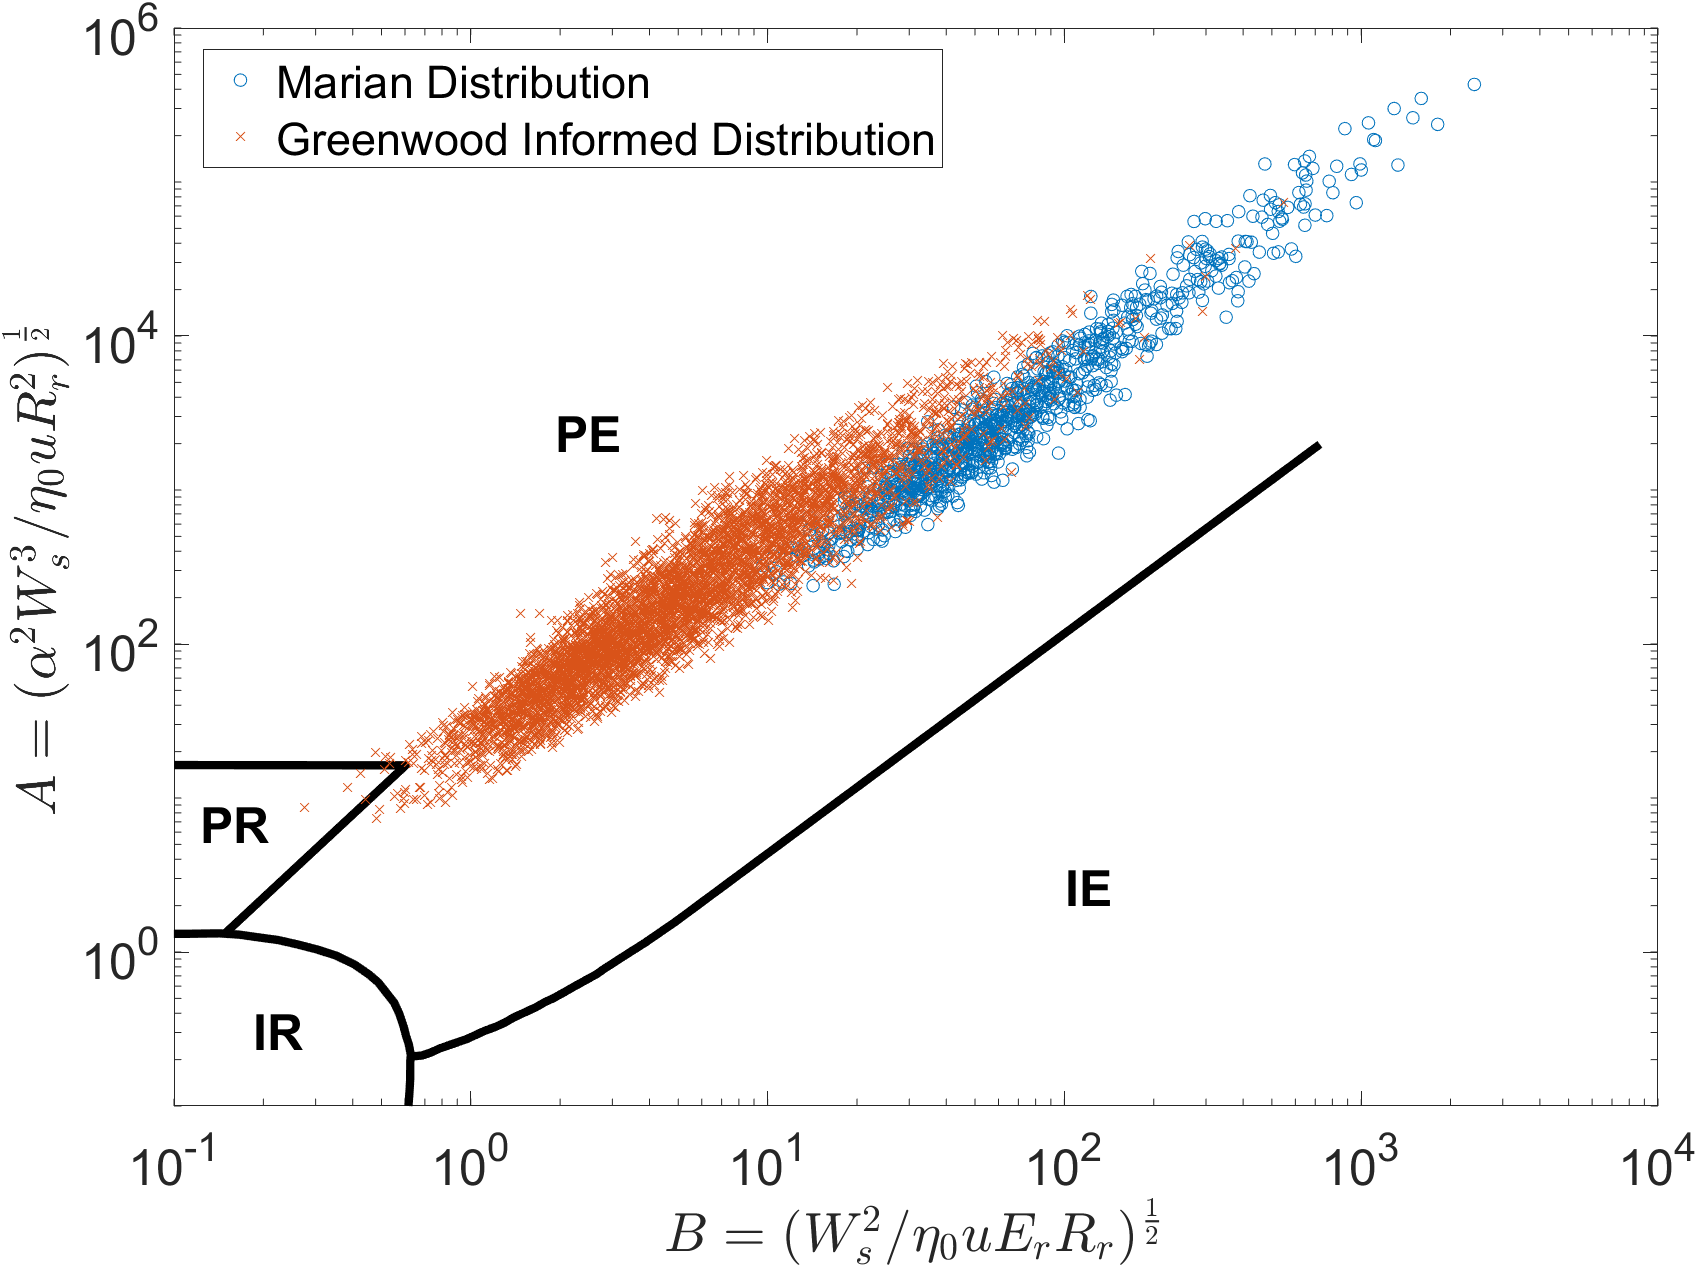
\includegraphics[width=150mm]{ANN_Explicit_MarianvsGreenwood.png}
	\caption{Greenwood informed training data vs Marian et al. \cite{Marian2022}.}
	\label{Greenwood informed training data vs Marian et al.}
\end{figure} 

\begin{table*}
	%\captionsetup{justification=centering}
	\caption{Range of ANN film thickness calculation parameters}
    \label{Range of ANN film thickness calculation parameters}
	\centering
	\renewcommand{\arraystretch}{1.5}%
	\begin{tabular}{|P{0.4\textwidth}|P{0.15\textwidth}|P{0.15\textwidth}|P{0.15\textwidth}|}
		\hline
		\textbf{Parameter} & \textbf{Unit} & \textbf{Minimum} & \textbf{Maximum} \\ [0.5ex]
		\hline
		Load & $N$ & 150 & 5000 \\ [0.5ex]
		\hline
		Entraining Velocity & $m/s$ & 0.6 & 30 \\ [0.5ex]
		\hline
		Reduced Radius & $m$ & 0.0001 & 0.02 \\ [0.5ex]
		\hline
		Reduced Elastic Modulus & $GPa$ & 200 & 250 \\ [0.5ex]
		\hline
		Pressure-Viscosity Coefficient & ${GPa}^{-1}$ & 10 & 30 \\ [0.5ex]
		\hline
		Reference Viscosity & $Pa.s$ & 0.0005 & 0.1 \\ [0.5ex]
		\hline
		Maximum Density & ${kg}/{m}^3$ & 7750 & 8050 \\ [0.5ex]
		\hline
		Poisson's Ratio & $-$ & 0.3 & 0.35 \\ [0.5ex]
		\hline
		Contact Length & $m$ & 0.001 & 0.050 \\ [0.5ex]
		\hline
		
	\end{tabular}
\end{table*}

\textbf{CHECK THIS}The numerical solution database can also benefit from explicit parallelisation ie. use of multiple computational cores of the CPU. When using MBD solvers implicitly it is not possible to use explicit parallelisation since a particular time step is dependent on the present timestep as well as on data of the same timestep. The ANN functionality in turn can be embedded with an implicit MBD computation environment to significantly improve the computation times without the need of explicit parallelisation despite benefitting from it indirectly. 

\subsubsection{ANN Structure}
Normalization of the input and target parameters is first performed using min-max normalisation function:

\begin{equation}
	\tilde{x}=\frac{x-x_{\min }}{x_{\max }-x_{\min }}(u-l)+u
\end{equation}

Where $u$, and $l$ represent the upper and lower normalized unit values of 1 , and -1 respectively. The dimensional target input value is denoted by $x$, and the final normalised input or output parameter of the ANN is denoted by $\tilde{x}$. In order to dimensionalise the output layer, $x_{\max }, x_{\min }$ must be stored as a variable.

The dataset is divided into three sets: the training set, the validation set, and the test set, each containing 70~$\%$, 15~$\%$ and 15~$\%$ of the training data respectively:

\begin{enumerate}
	\item Training Set: The training set is the portion of the dataset used to train the ANN, containing the input data and the corresponding output data. As aforementioned, the ANN adjusts the internal parameters based on this data to learn the underlying patterns and relationships.
	\item Validation Set: The validation set is used to tune the performance of the ANN during the training process. It is an independent dataset that the network has not seen before, allowing for the evaluation of its generalization capabilities. The network's performance on the validation set is monitored during training to make decisions on adjusting hyperparameters (number of hidden layers, neurons per hidden layer, activation functions etc.) or stopping the training process to prevent overfitting.
	\item Test Set: The test set is a completely independent dataset that is not used during training or validation. It is used to assess the final performance and generalization ability of the trained ANN. By evaluating the network on unseen data, the test set provides an unbiased estimate of the model's performance in actual use.
\end{enumerate}

A limit of 1000 epochs was also implemented. This limits the ANN to 1000 full iterations through the entire training set during training. This was found to be sufficient to improve accuracy whilst preventing overfitting of the data.

During back propagation of the ANN, the Mean Squared Error (MSE) was used to evaluate the network's performance:

\begin{equation}\label{MSE}
	M S E=\frac{1}{N} \sum_{i=1}^N\left(t_i-y_i\right)^2
\end{equation}

The total number of training points being trained, validated or tested is denoted by $N$. 

To assess the goodness of fit of the ANN, the statistical metric $R^2$ known as the coefficient of determination was used. This measured the proportion of variance in the dependant variable (output film thickness) that is predictable from the input variables (Table \ref{Range of ANN film thickness calculation parameters}) in the model. This value ranges from 0 to 1, with a higher value indicating the best fit of the model to the data. This was post-processed after training and is calculated as follows \cite{Marian2022}:

\begin{equation}\label{R-squared}
	R^2=1-\frac{\sum_{i=1}^N\left(t_i-y_i\right)^2}{\sum_{i=1}^N\left(y_i-\bar{y}\right)^2}
\end{equation}

where $t_i$ and $y_i$ are the target and predicted value respectively. $\overline{\mathrm{y}}$ is the mean of the target sample. The numerator of the fraction is the sum of the squares of residuals, which represents that variation in target variable that is not explained by the model. The denominator is the total sum of squares and represents the total variation in the target variable. 

Activation functions:

Activation functions are mathematical functions that are applied to the output of each neuron in a layer of the neural network. These introduce non-linearity which allow the network to learn complex input-output relationships. Activation functions help determine the  output of a neuron based on the weighted sum of its inputs.

As suggested per \cite{Marian2022}, suitable activation functions for the hidden layers are as follows:

\begin{itemize}
	\item Sigmoid (logistic): This function transforms the input values into a range between 0 and 1. It has continuously differentiable smooth S-shaped curve and is given by the following formula \cite{Han1995}:
	
	\begin{equation}\label{Logistic sigmoid}
		\log \operatorname{sig}(x)=\frac{1}{1+e^{-x}}
	\end{equation} 

	Sigmoid functions are commonly used in the hidden layers of ANNs, however may suffer from the "vanishing gradient" problem where the partial derivative reaches zero \cite{Sharma2020}, leading to slower convergence during training.

	\item ReLU (Rectified Linear Unit): This function is the most commonly used activation function. It outputs the input value directly if it is positive, and zero otherwise. The mathematical definition is:
	
	\begin{equation}\label{ReLU}
		\operatorname{ReLU}= \begin{cases}x, & x \geq 0 \\ 0, & x \leq 0\end{cases}
	\end{equation}

	The gradient is 1 when the neuron is activated, and zero when it is deactivated. This function is computationally efficient and addresses the vanishing gradient problem to an extent \cite{Sharma2020}.
	
	\item Tanh (Hyperbolic Tangent): The hyperbolic tangent or tanh function is also commonly used. It is defined as:
	
	\begin{equation}\label{Hyperbolic tangent}
		\tanh (x)=\frac{2}{1+e^{-2 x}}-1
	\end{equation}

	The formulation and behaviour is very similar to sigmoid. It produces values which range from -1 to 1, having a centred mean around zero. Like sigmoid, this also experiences vanishing gradients.
	
\end{itemize}

A simple linear activation was used on the output.

The training data size was varied (600, 1000, 2000 and 5000) to observe the its effect on the quality of the prediction.

Early stopping and regularisation was used to prevent statistical overfitting during training. Early stopping halts the training process before the model reaches the maximum number of epochs. This is done by monitoring the performance (MSE (Equation \ref{MSE})) of the network against the validation set during training. One the performance reaches a plateau, or begins to degrade, the training is stopped early. Regularisation adds additional constraints to the learning process. It modifies the performance criteria by accounting for the change in mean square of the network weights and biases (MSW (Eq. \ref{MSW})). By applying an adjustment factor, denoted as $\gamma^{\prime}$, the weights and biases can be reduced during propagation (Eq. \ref{MSE adjusted}) , thus mitigating the risk of overfitting and improving the network's generalization capability.

\begin{equation}\label{MSW}
	M S W=\frac{1}{N} \sum_{j=1}^N w_j^2
\end{equation}

\begin{equation}\label{MSE adjusted}
	M S E_{r e g}=\gamma^{\prime} * M S W+\left(1-\gamma^{\prime}\right) * M S E
\end{equation}

\subsubsection{Explicit Roller Bearing Implementation}
The same FMBD model used in Chapter \ref{Lubricated FMBD} was used for this study. The shaft was modelled as a rigid body, and loading was purely static in one radial direction to remove the influence of dynamic effects. The shaft is constrained to one rotational and two lateral degrees of freedom. Bearing properties and operating conditions are shown in Table \ref{Roller bearing parameters} and Table \ref{Operating Conditions} respectively.

\begin{table*}
	%\captionsetup{justification=centering}
	\caption{Roller Bearing Parameters}
	\label{Roller bearing parameters}
	\centering
	\renewcommand{\arraystretch}{1.5}%
	\begin{tabular}{|c|c|}
		\hline
		\ \textbf{Parameter} & \textbf{Value} \\ [0.5ex]
		\hline
		Inner race diameter & 31.5 $mm$ \\ [0.5ex]
		\hline
		Roller diameter & 7.5 $mm$ \\ [0.5ex]
		\hline
		Roller length & 15 $mm$ \\ [0.5ex]
		\hline
		Number of rollers & 12 \\ [0.5ex]
		\hline
		Radial interference & 5 $\mu \mathrm{m}$ \\ [0.5ex]
		\hline
		Young's modulus & 218 $GPa$ \\ [0.5ex]
		\hline
		Poisson's ratio & 5 $0.3$ \\ [0.5ex]
		\hline
	\end{tabular}
\end{table*}

\begin{table*}
	%\captionsetup{justification=centering}
	\caption{Operating Conditions}
	\label{Operating Conditions}
	\centering
	\renewcommand{\arraystretch}{1.5}%
	\begin{tabular}{|c|c|}
		\hline
		\ \textbf{Parameter} & \textbf{Value} \\ [0.5ex]
		\hline
		Radial force & 2500 $N$ \\ [0.5ex]
		\hline
		Rotational velocity & 10~000$rpm$ \\ [0.5ex]
		\hline
	\end{tabular}
\end{table*}

The dynamic model was run explictly as a dry model, without the influence of the EHL film at the roller-race contacts. The kinematic and dynamic results required for input to the ANN are then extracted at each time step. Results were generated for an individual element completing one complete orbit around the bearing. Extracted results include roller load per unit length, reduced radius of the contact between the roller and inner-race, and the contact entrainment velocity.

The loading pattern is cyclic in nature as the roller enters and exits the most highly loaded region of the bearing, corresponding to the force vector applied to the inner race. Sufficient preload ensures constant contact between elements and raceways so that the regime does not deviate from EHL. The contact reduced radius and entrainment speed do not change throughout the orbit as they are a function of bearing geometry and constant operating speed.

\begin{figure}
	\centering
	\begin{subfigure}[b]{0.9\textwidth}
		\centering
		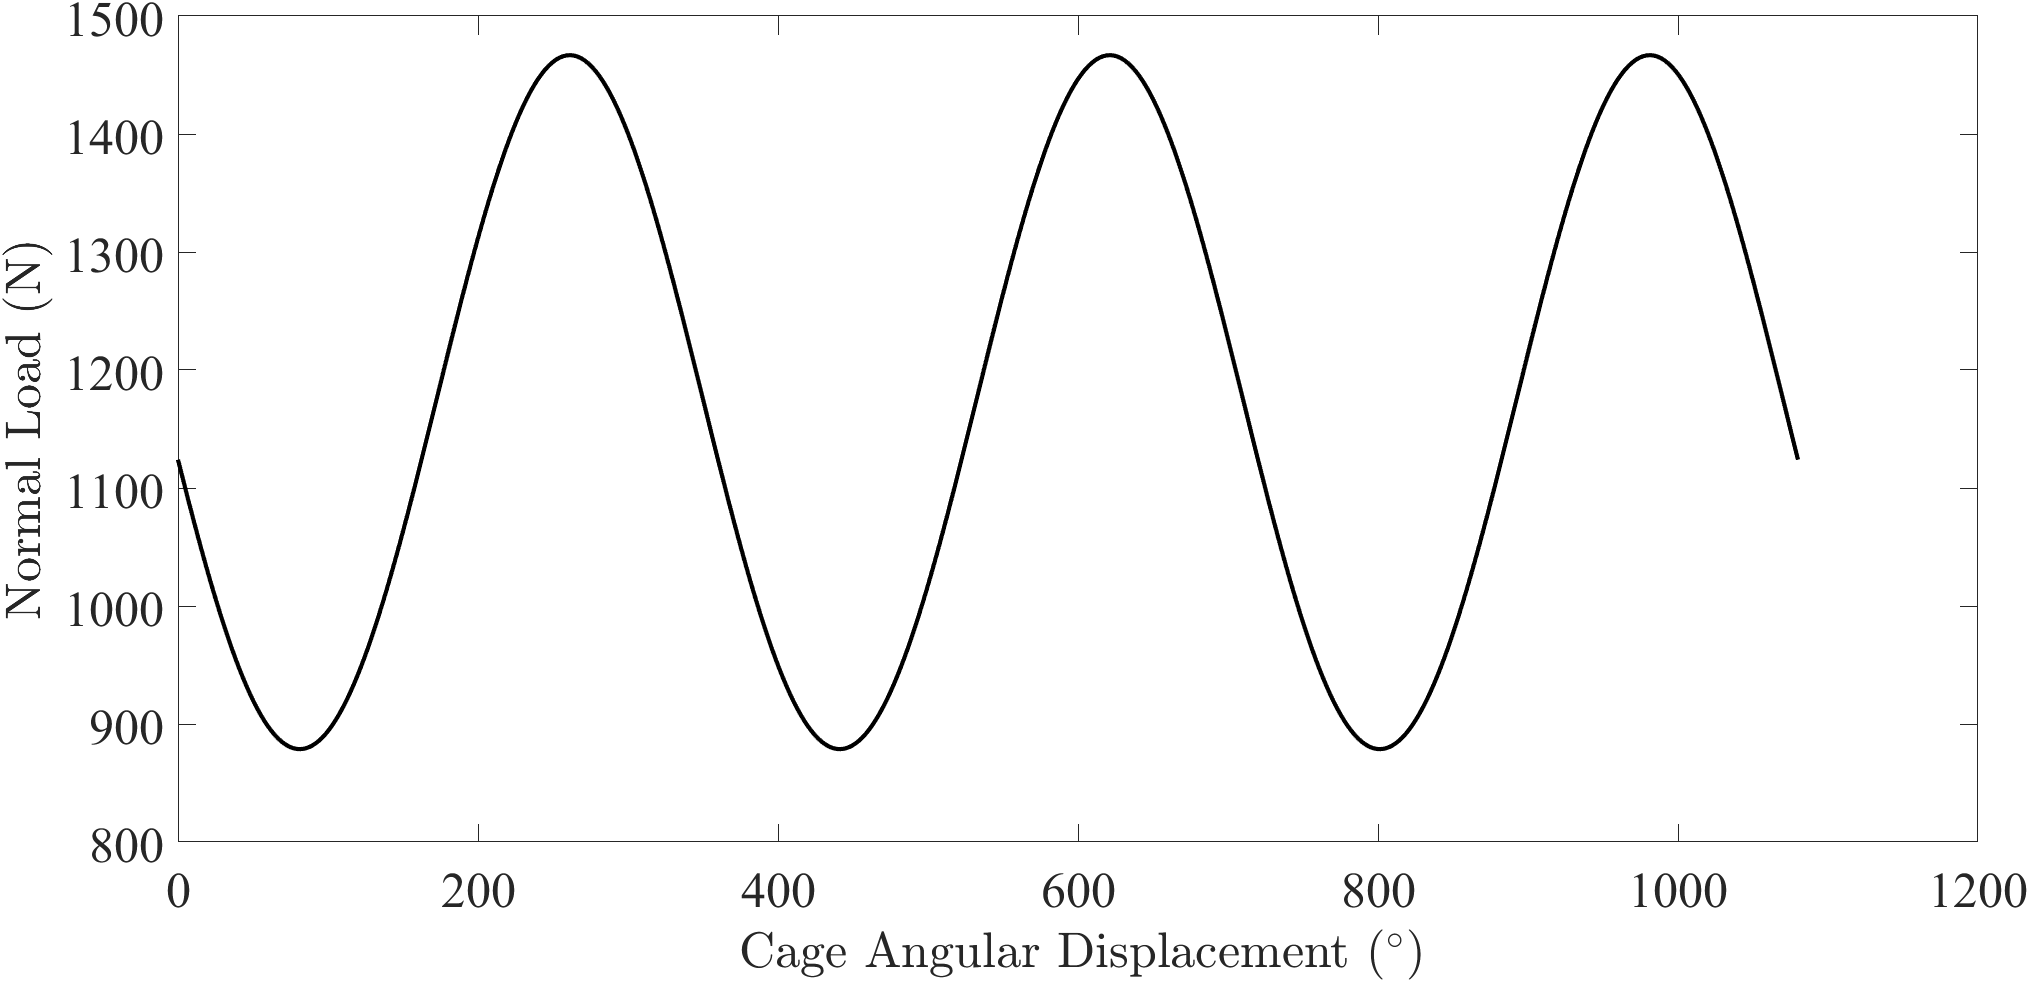
\includegraphics[width=\textwidth]{ANN_Explicit_Bearing Normal Load.png}
		\caption{}
		\label{Contact Normal Load ANN}
	\end{subfigure}
	\hfill
	\begin{subfigure}[b]{0.9\textwidth}
		\centering
		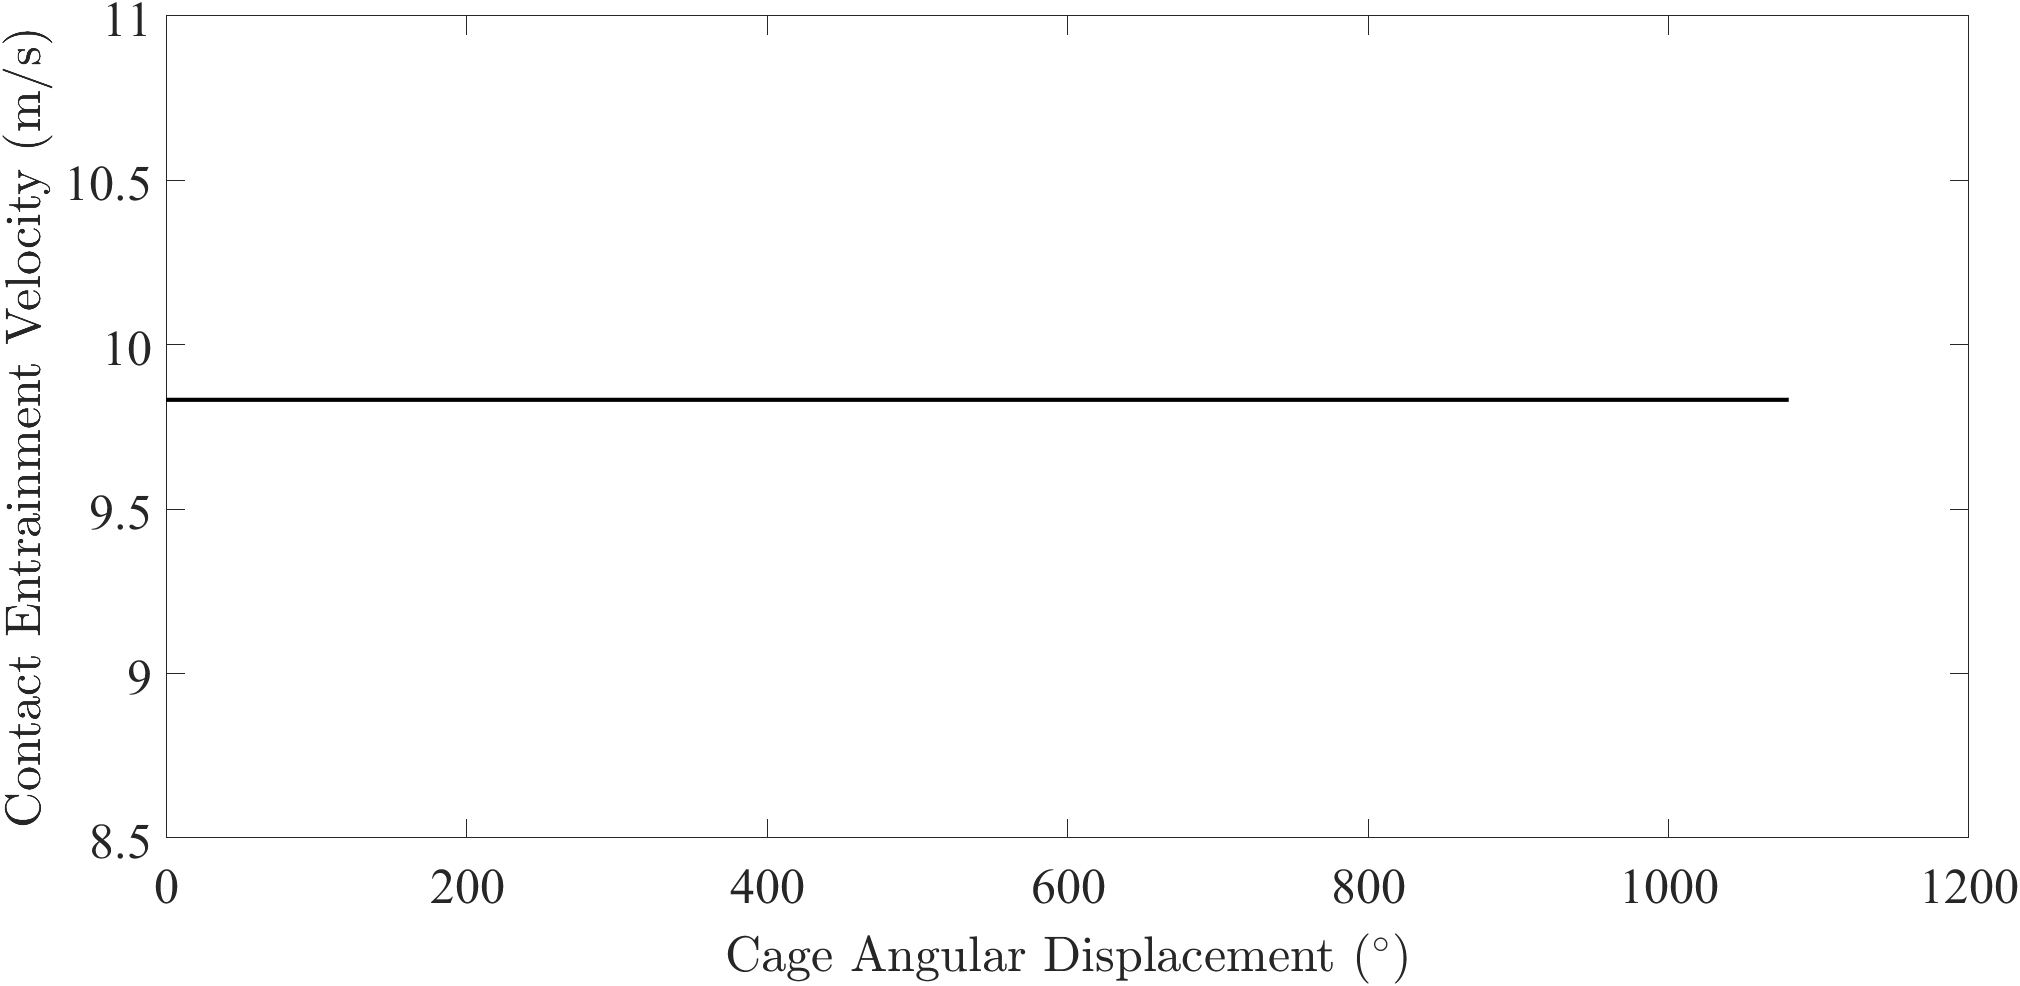
\includegraphics[width=\textwidth]{ANN_Explicit_Bearing Entrainment Velocity.png}
		\caption{}
		\label{Contact Entrainment ANN}
	\end{subfigure}
	\hfill
	\begin{subfigure}[b]{0.9\textwidth}
		\centering
		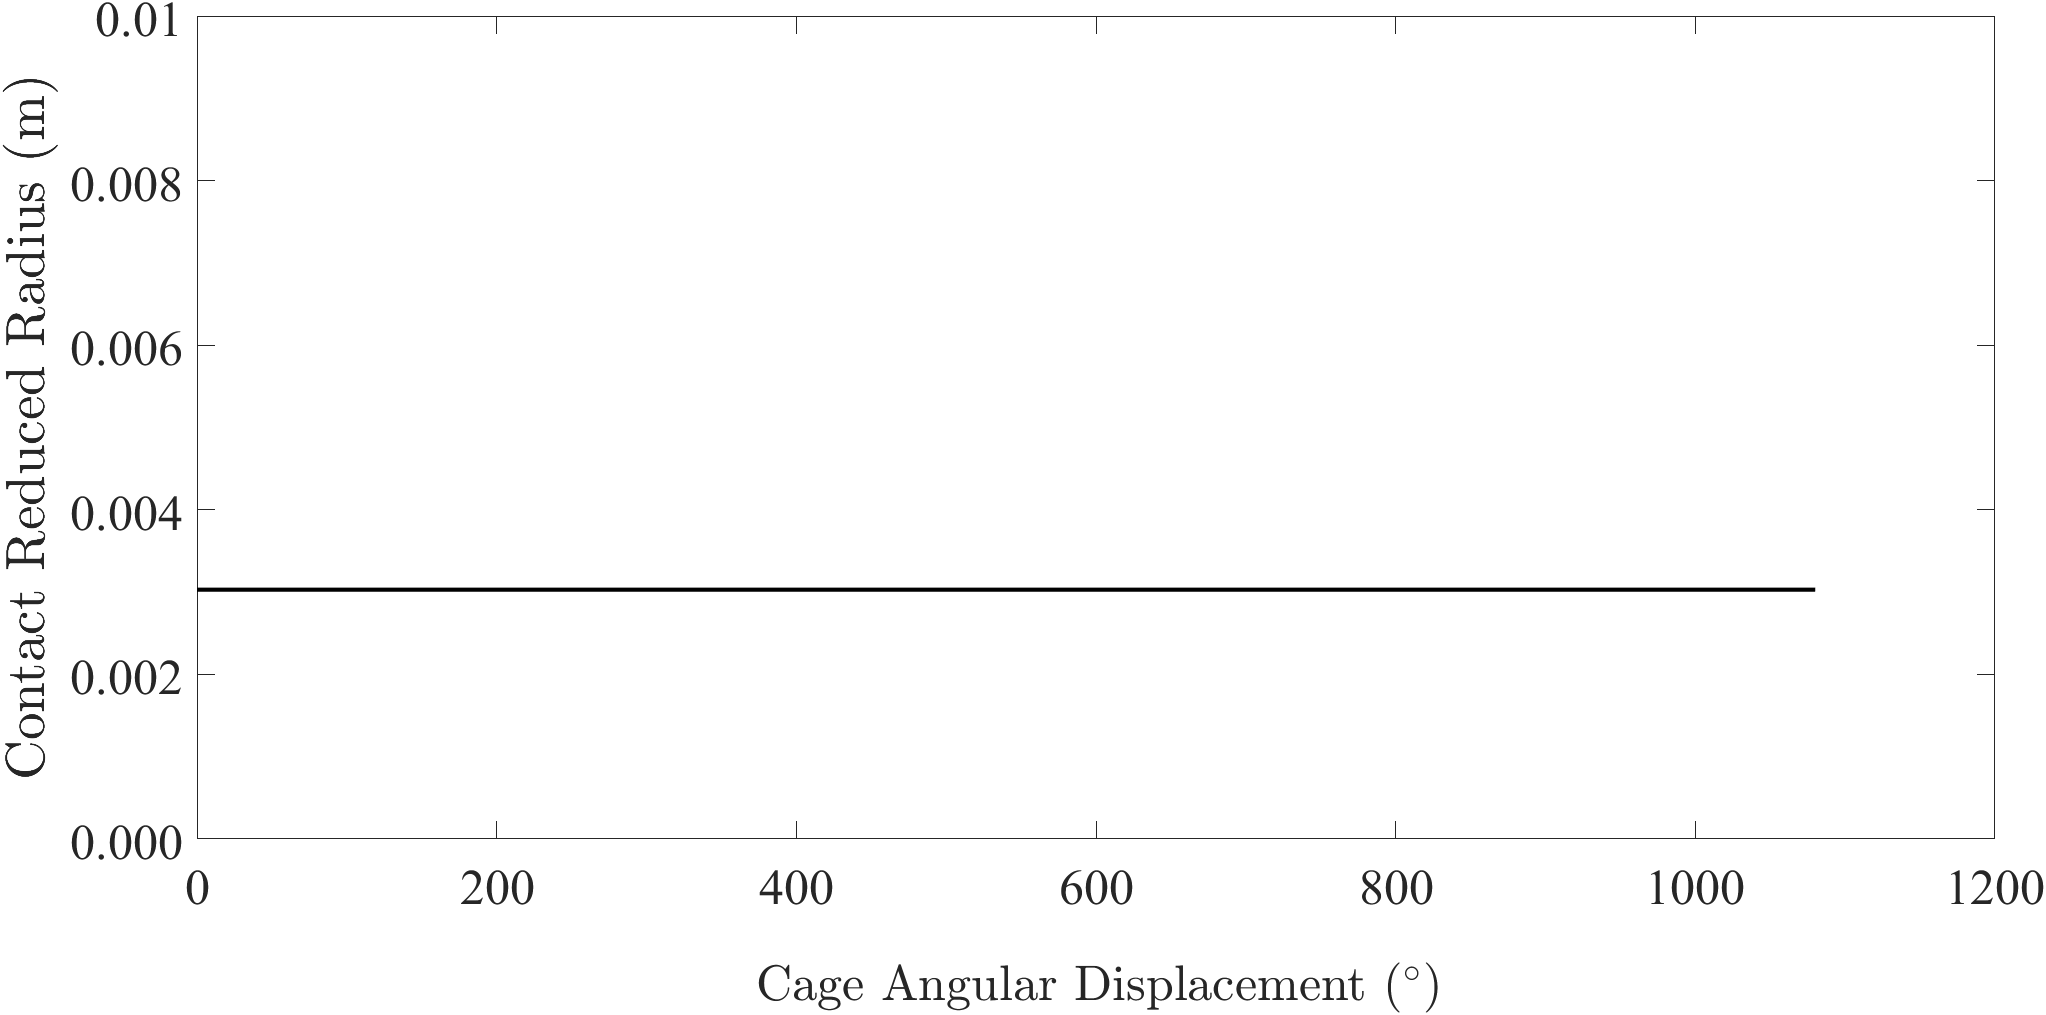
\includegraphics[width=\textwidth]{ANN_Explicit_Bearing Reduced Radius.png}
		\caption{}
		\label{Contact Reduced Radius ANN}
	\end{subfigure}
	\caption{Individual rolling element input values to ANN : a) Contact load, b) Contact entrainment velocity, c) Contact reduced radius}
	\label{Individual rolling element input values to ANN}
\end{figure}








\section{Results and Discussion}

The following data was obtained using consumer grade hardware with the following specifications: 
Intel® Core™ i7-9750H CPU 6 cores @ 2.60GHz, 32GB RAM; GPU: NVDIA GeForce GTX 1650.

The same hardware was used for both the full numerical and the ANN solutions to provide performance comparisons and assess the suitability of ANNs for film thickness calculations in FMBD solvers.

\subsubsection{ANN Structure and Performance}

The 1D EHL model presented in Section \ref{1D EHL Model} was used to generate the numerical database for training the ANN. Each numerical solution and hence training point took an average of 5.88~$s$. The construction of the entire database on a single core therefore has a wall time of between 58.8~$min$ and 489~$min$ for 600 and 5000 points respectively. This wall time is purely for baseline comparisons, and can be significantly improved using parallelisation across multiple cores.

A parameter study was conducted to determine the optimal structure for the ANN. Over 500 different structures were tested using the same input data. This involved varying the hyperparameters: the number of hidden layers varied from one to four, and the number of neurons from ten to twenty. The three aforementioned activation functions were explored in different hidden layer configurations. This included a combination of hyperbolic tangent in the hidden layers, with the final layer utilizing a logistic tangent function. For each configuration, the values of $R^2$ (coefficient of determination) and the training completion time were carefully documented.

Tables \ref{LogSig_table}-\ref{ANN_Explicit_LogSig_5000_table} present the $R^2$ values obtained from 600 data points, considering different activation functions, number of layers, and neurons. Among the activation functions tested, the ReLU function consistently underperformed when compared to the logistic sigmoid and hyperbolic tangent functions across all network structures. It is important to acknowledge that there is a slight variability in the performance of the network with each new training session. However, it is worth noting that the optimum number of layers, similar to tribological applications of ANNs \cite{Marian2021}, was found to be between two and three.

\begin{table}
	\caption{$R^2$ performance of ANN structures using 600 data points and a LogSig activation function}
	\label{LogSig_table}
	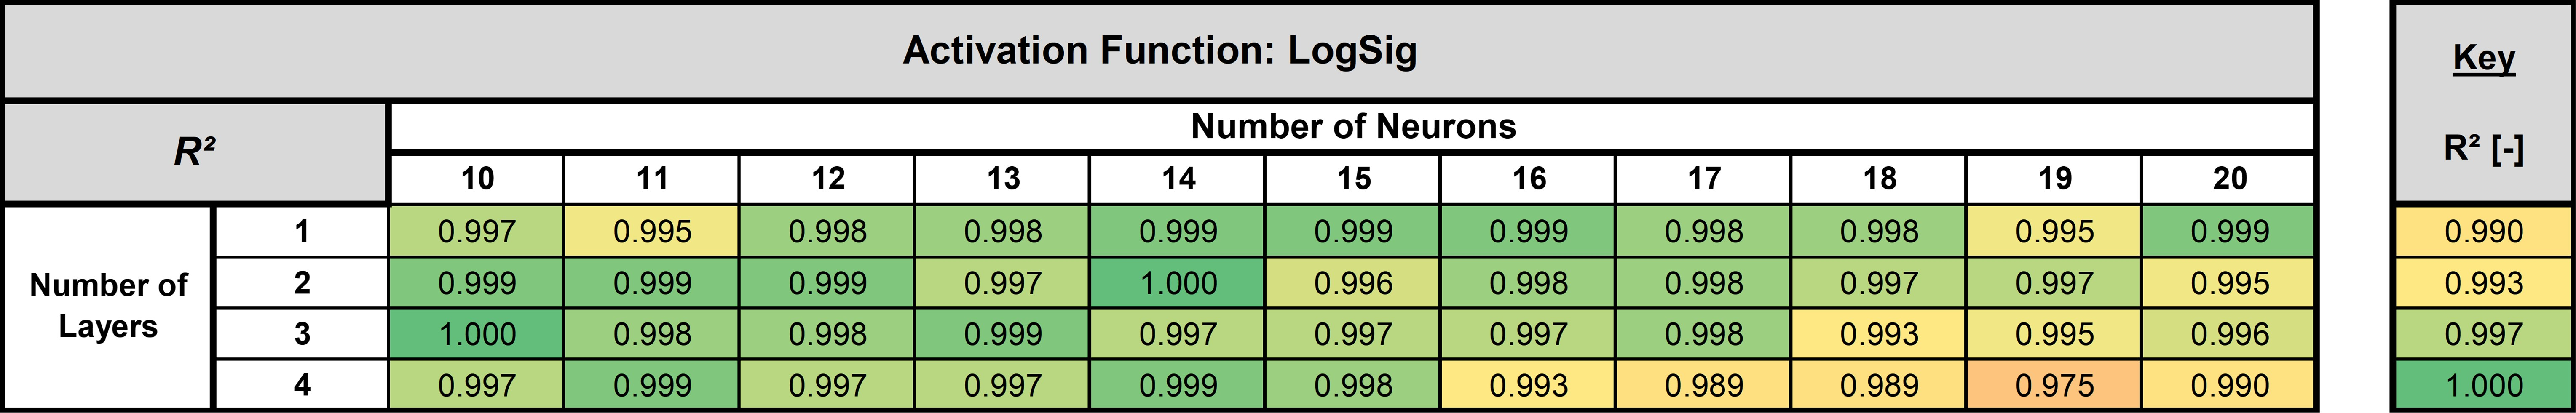
\includegraphics[width=\linewidth]{ANN_Explicit_ActFun_LogSig.jpg}
\end{table}

\begin{table}
	\caption{$R^2$ performance of ANN structures using 600 data points and a Tanh activation function}
	\label{Tanh_table}
	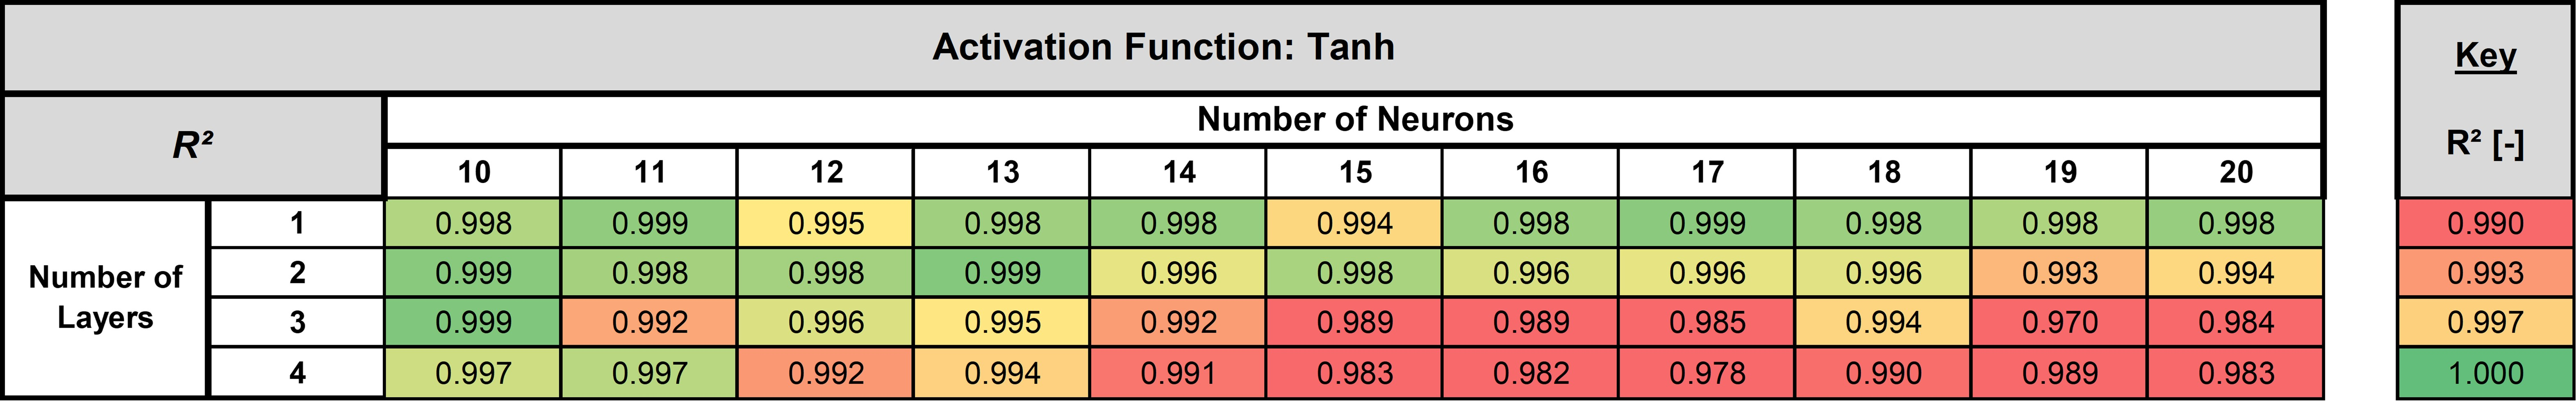
\includegraphics[width=\linewidth]{ANN_Explicit_ActFun_Tanh.jpg}
\end{table}

\begin{table}
	\caption{$R^2$ performance of ANN structures using 600 data points and a Tanh activation function}
	\label{ReLU_table}
	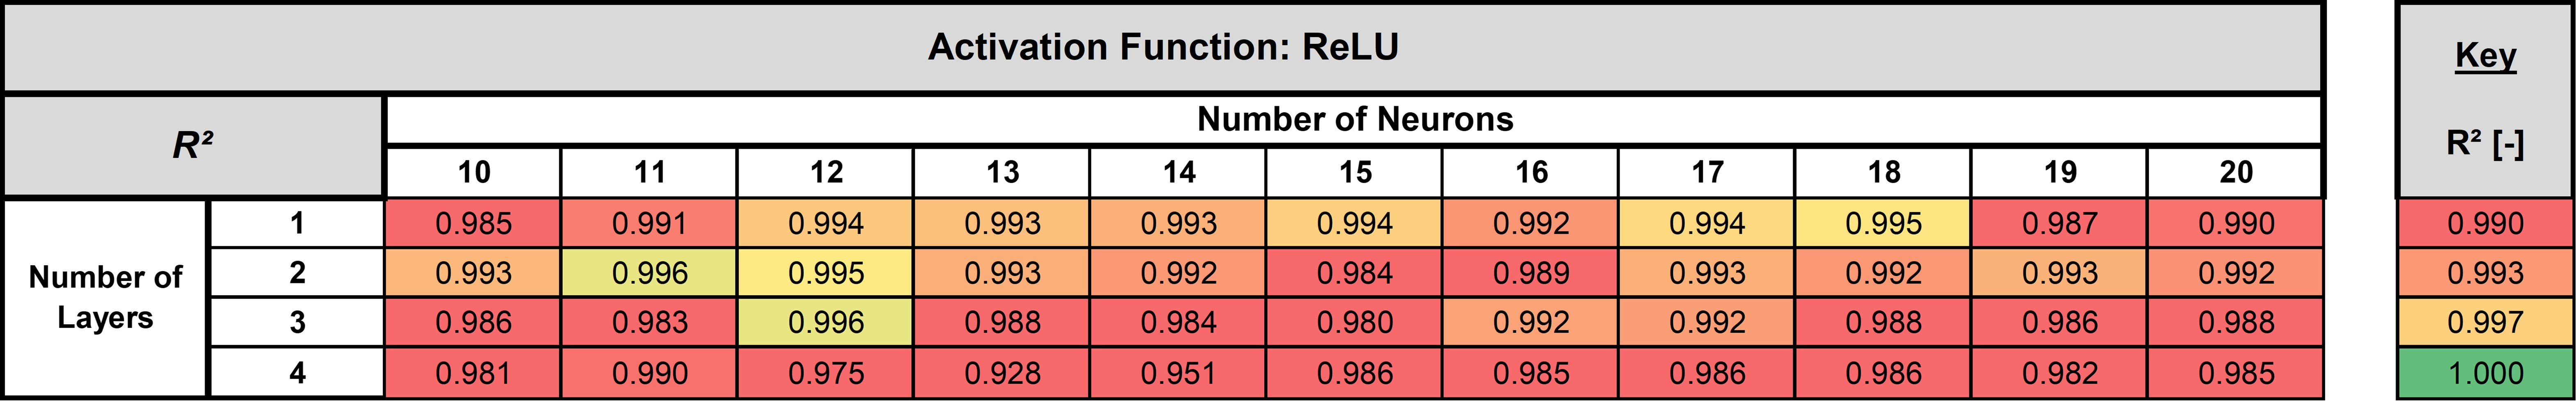
\includegraphics[width=\linewidth]{ANN_Explicit_ActFun_ReLU.jpg}
\end{table}

\begin{table}
	\caption{Training time of ANN structures with LogSig activation function and 600 data points}
	\label{ANN_Explicit_LogSig_600_table}
	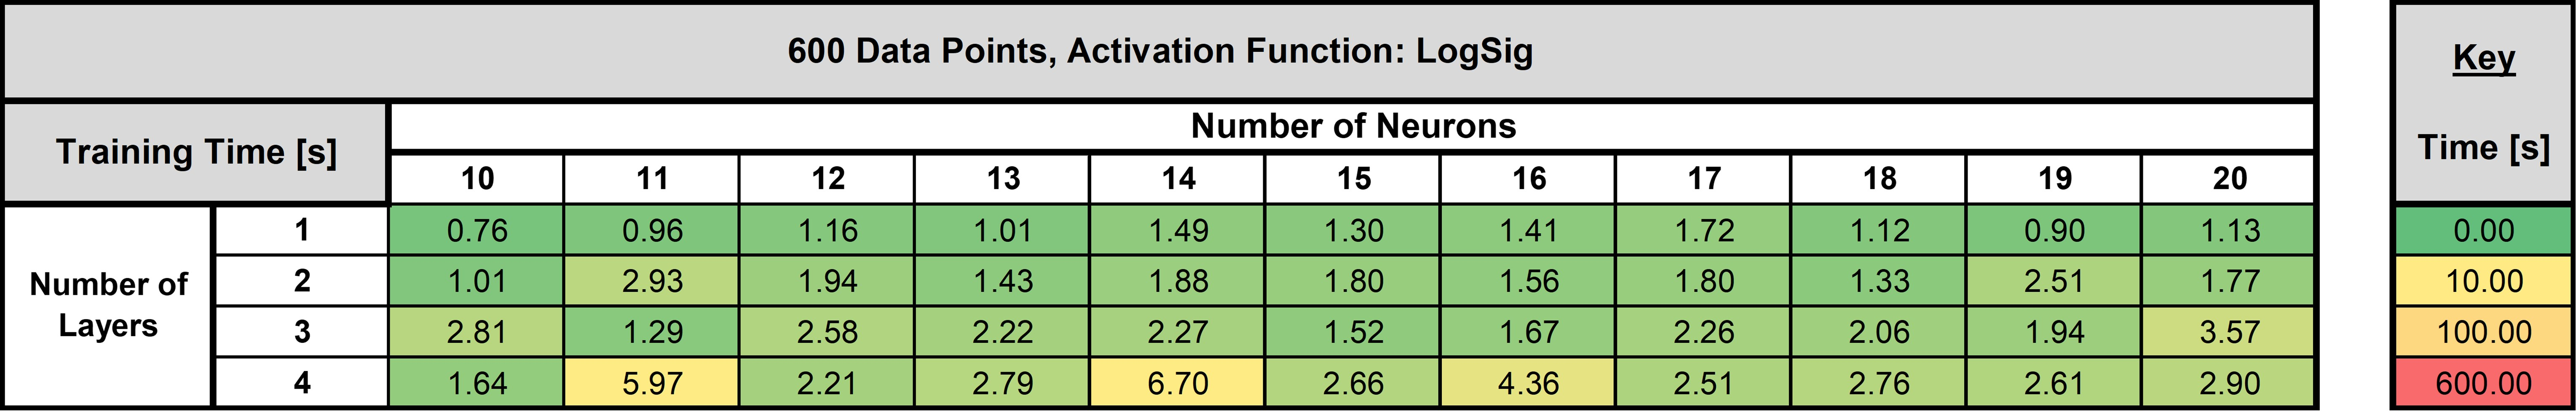
\includegraphics[width=\linewidth]{ANN_Explicit_LogSig_600.jpg}
\end{table}

\begin{table}
	\caption{Training time of ANN structures with LogSig activation function and 1000 data points}
	\label{ANN_Explicit_LogSig_1000_table}
	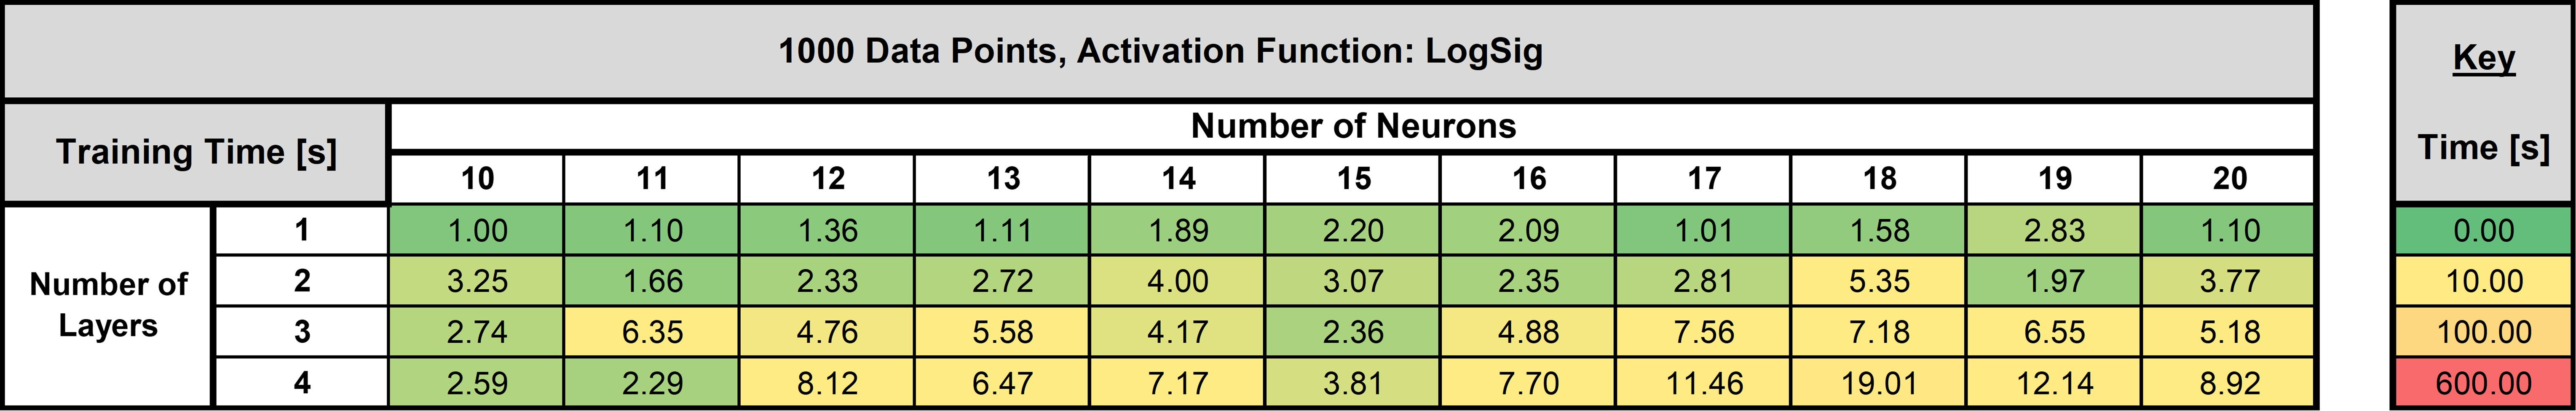
\includegraphics[width=\linewidth]{ANN_Explicit_LogSig_1000.jpg}
\end{table}

\begin{table}
	\caption{Training time of ANN structures with LogSig activation function and 2000 data points}
	\label{ANN_Explicit_LogSig_2000_table}
	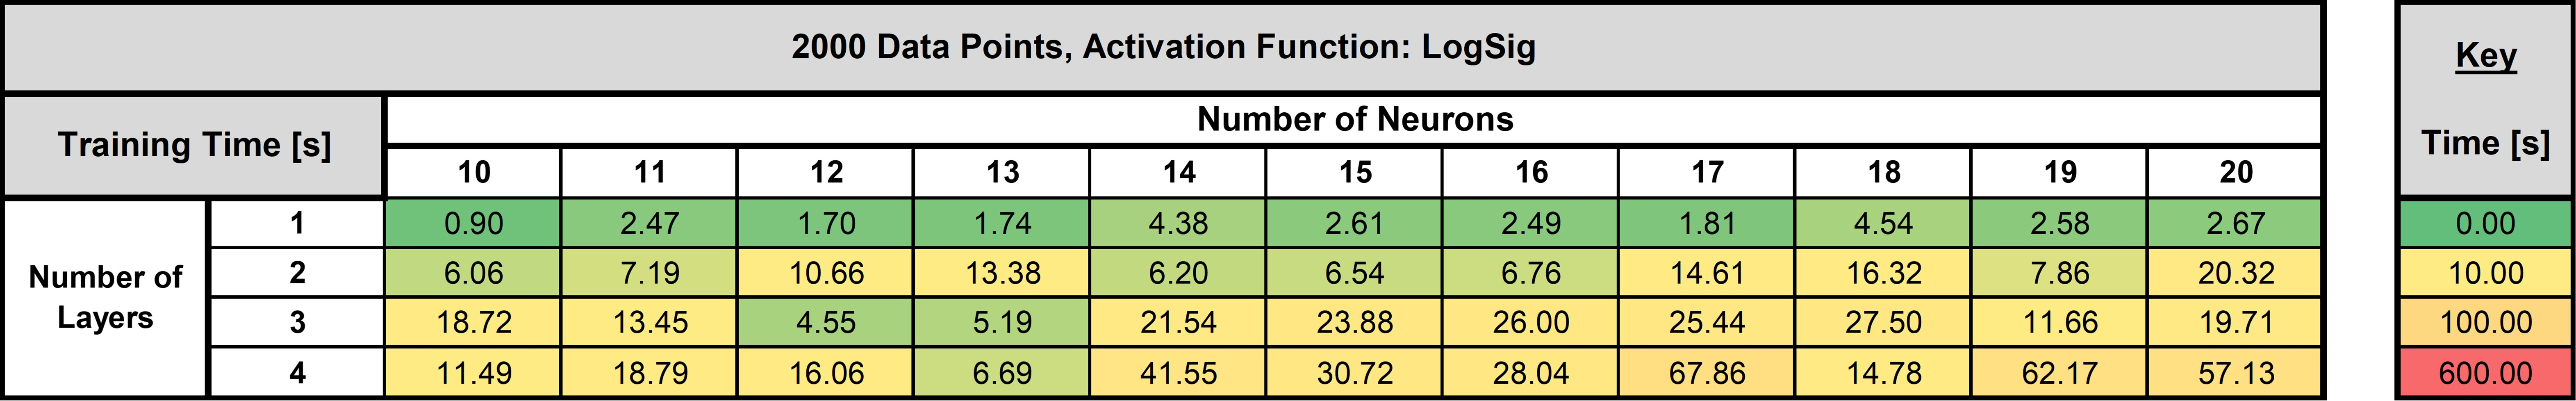
\includegraphics[width=\linewidth]{ANN_Explicit_LogSig_2000.jpg}
\end{table}

\begin{table}
	\caption{Training time of ANN structures with LogSig activation function and 5000 data points}
	\label{ANN_Explicit_LogSig_5000_table}
	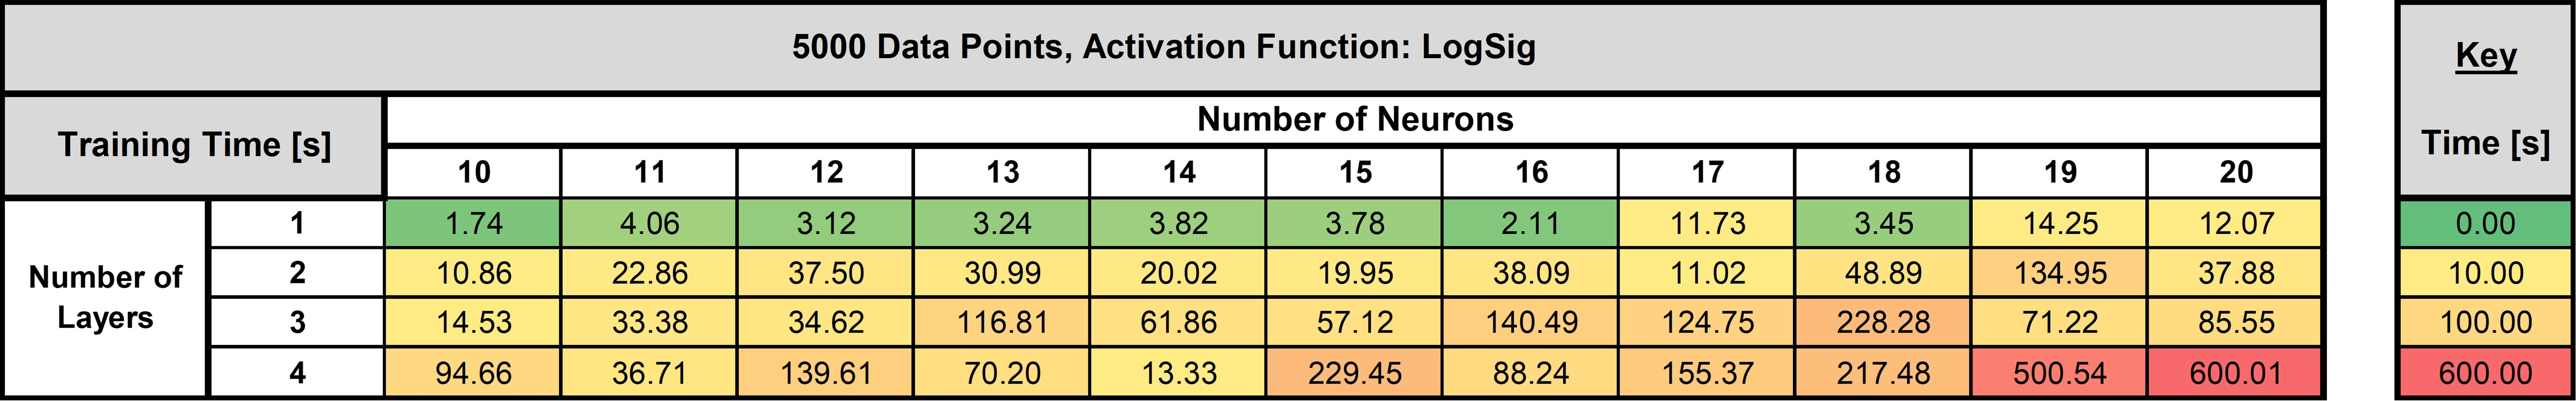
\includegraphics[width=\linewidth]{ANN_Explicit_LogSig_5000.jpg}
\end{table}

\begin{figure}
	\centering
	\begin{subfigure}[b]{0.49\textwidth}
		\centering
		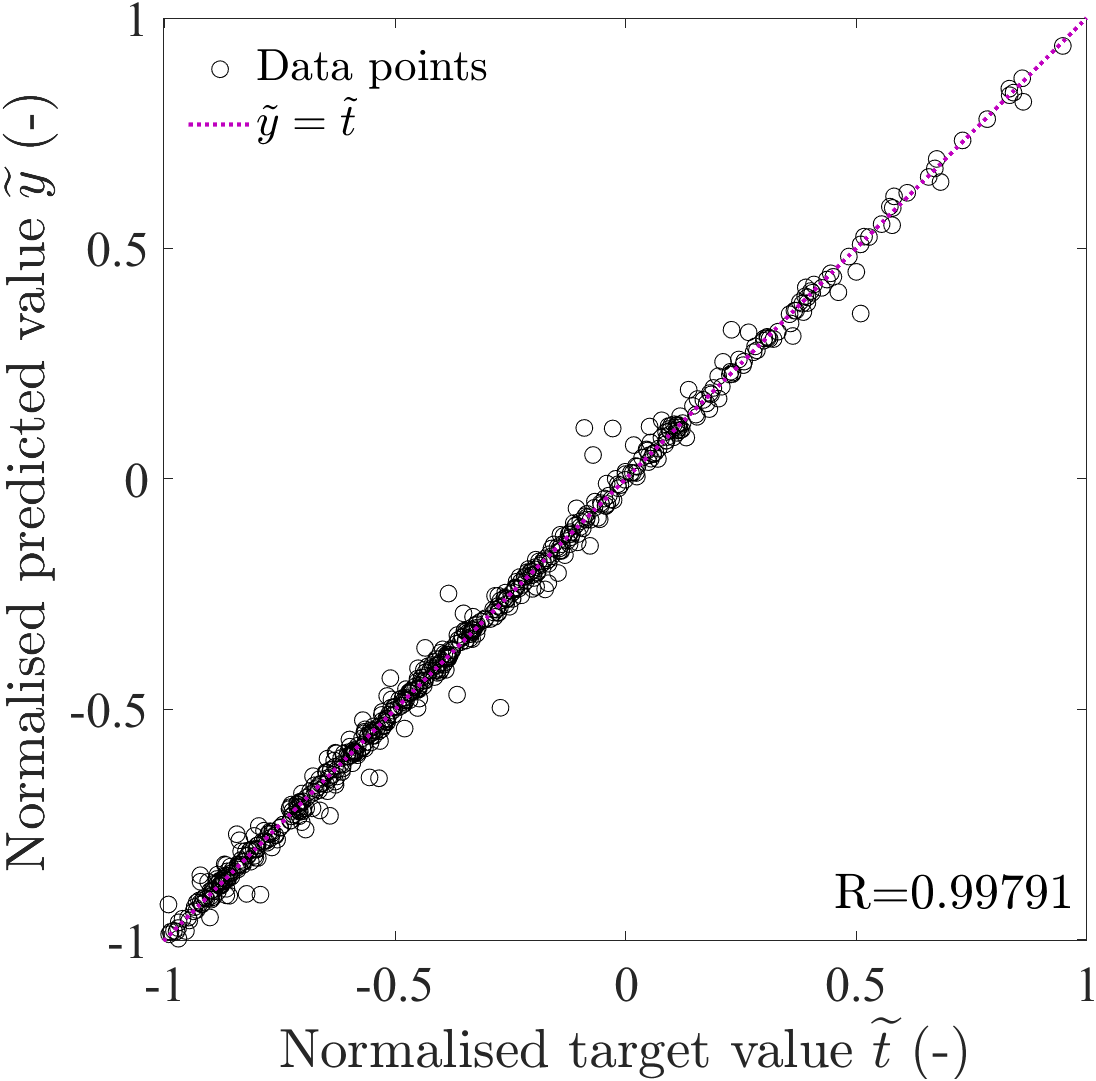
\includegraphics[width=\textwidth]{ANN_Explicit_600_Rval.png}
		\caption{}
		\label{600_Rval}
	\end{subfigure}
	\hfill
	\begin{subfigure}[b]{0.49\textwidth}
		\centering
		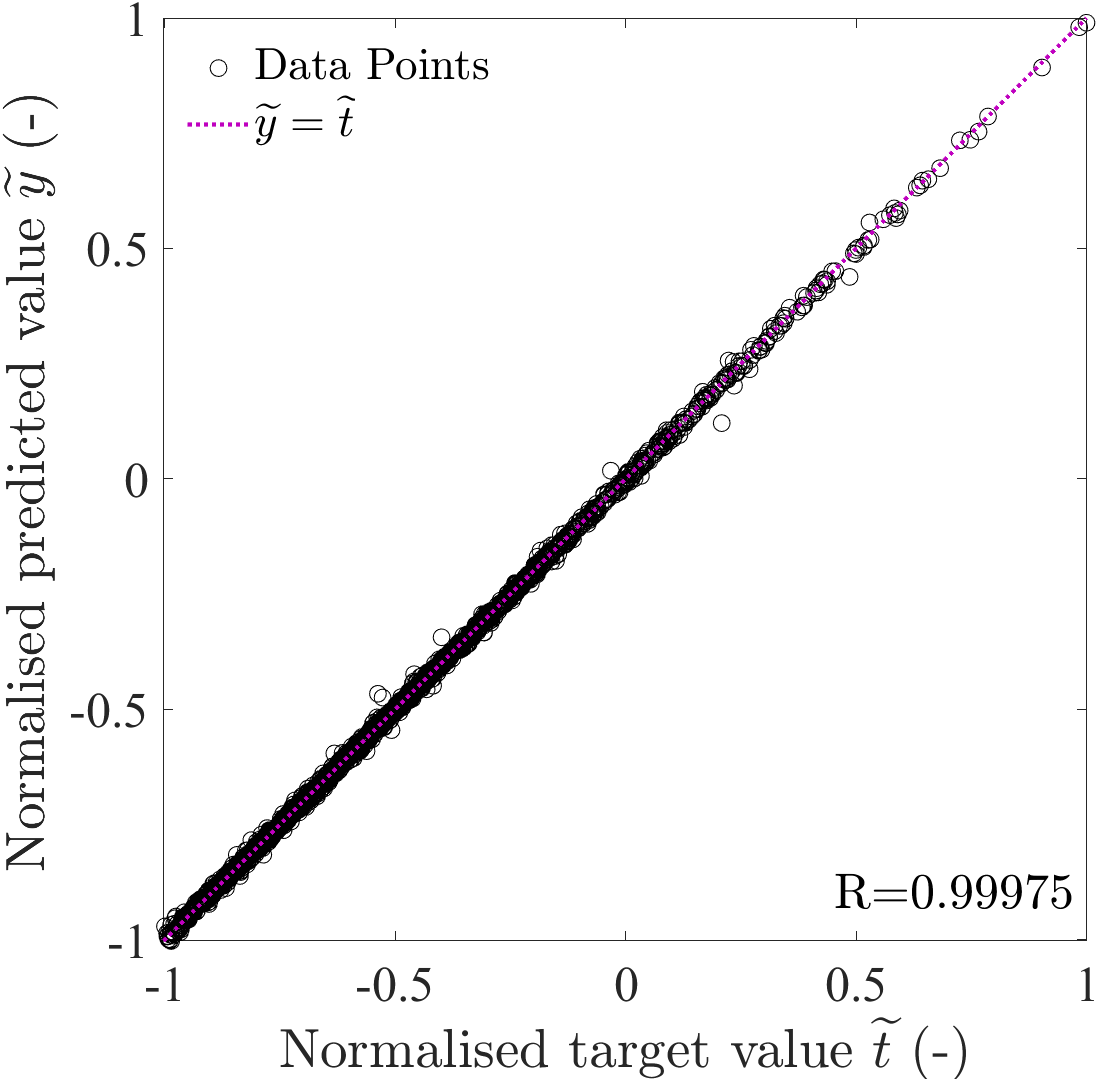
\includegraphics[width=\textwidth]{ANN_Explicit_1000_Rval.png}
		\caption{}
		\label{1000_Rval}
	\end{subfigure}
	\hfill
	\begin{subfigure}[b]{0.49\textwidth}
		\centering
		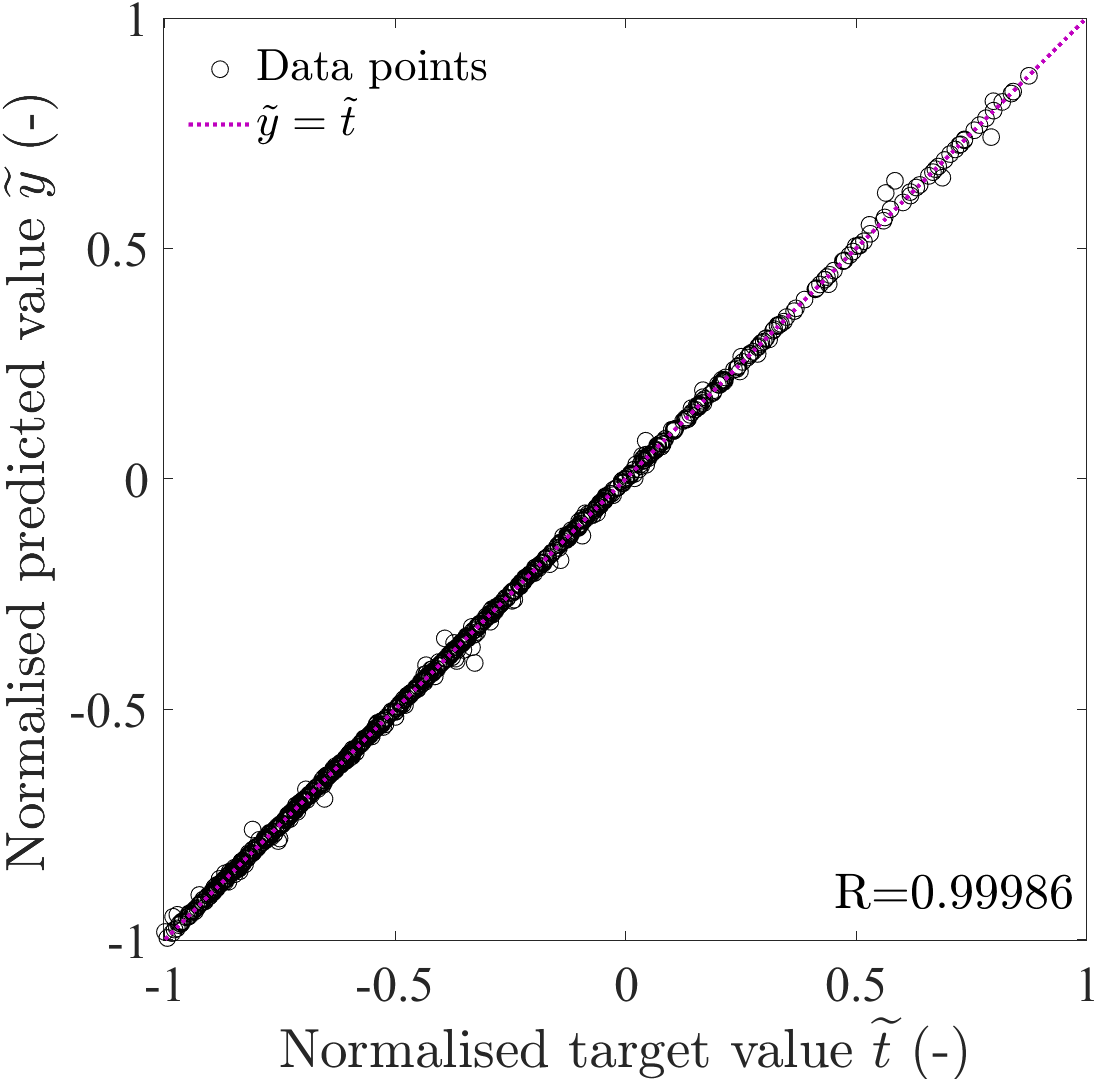
\includegraphics[width=\textwidth]{ANN_Explicit_2000_Rval.png}
		\caption{}
		\label{2000_Rval}
	\end{subfigure}
	\hfill
	\begin{subfigure}[b]{0.49\textwidth}
		\centering
		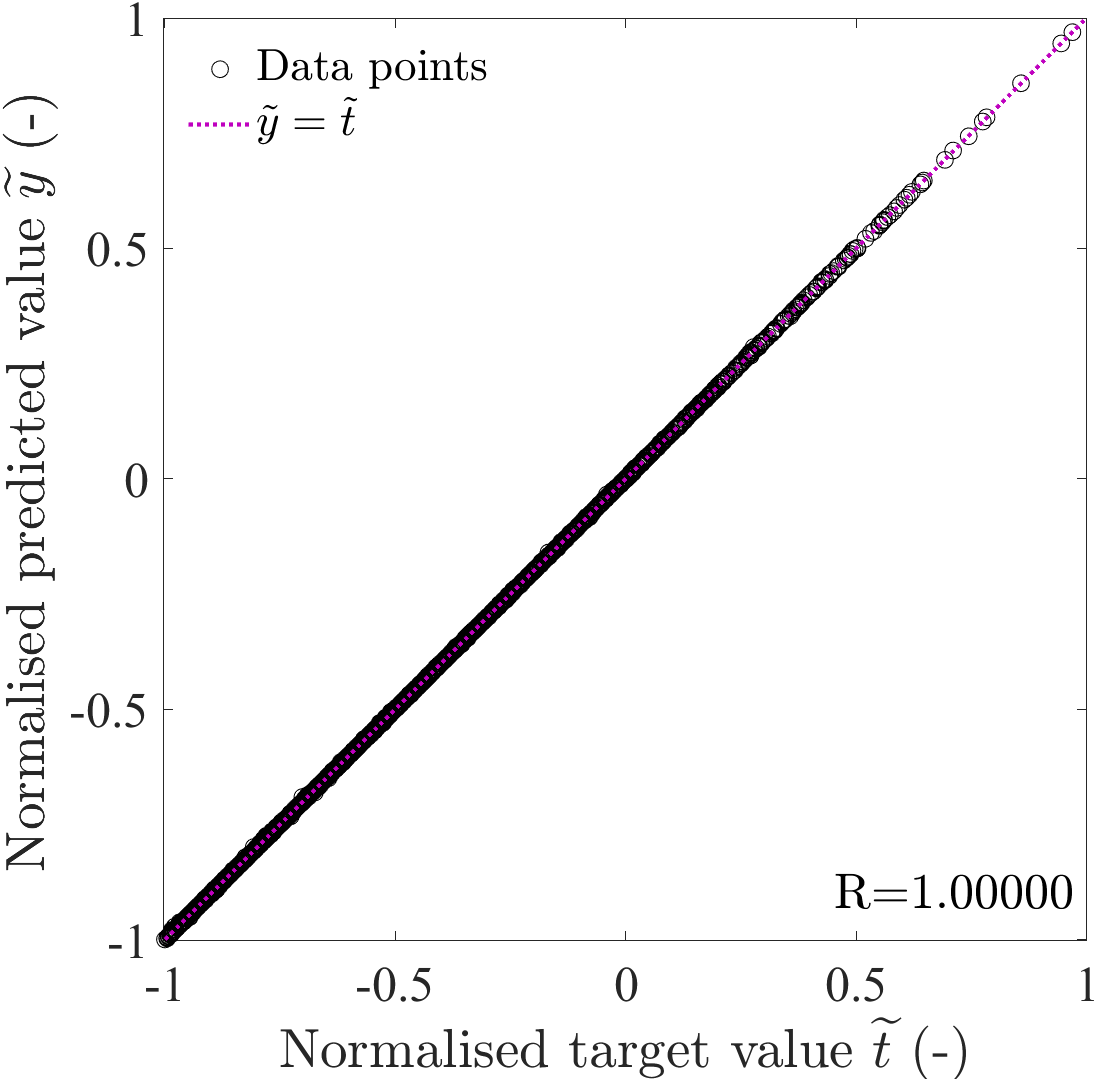
\includegraphics[width=\textwidth]{ANN_Explicit_5000_Rval.png}
		\caption{}
		\label{5000_Rval}
	\end{subfigure}
	\caption{$10-[14-14-14]_3-1$ using Hyperbolic Tangent activation function : a) 600 points, b) 1000 points, c) 2000 points, d) 5000 points}
	\label{$R^2$ performance of ANN structure}
\end{figure}







\subsubsection{Bearing Film Thickness Predictions}

After identifying suitable data set size and ANN structure, the ANN could then be compared to the analytical (Eq. \ref{DowsonToyodaCentralFilm}) and numerical (Section \ref{1D EHL Model}) methods of obtaining central film thickness at the roller-race contact. The operating conditions of the bearing were within the range of validity of the training data set. This is demonstrated in Figure \ref whereby the Greenwood parameters for the bearing operating points are overlayed on the training cloud.



\begin{figure}
	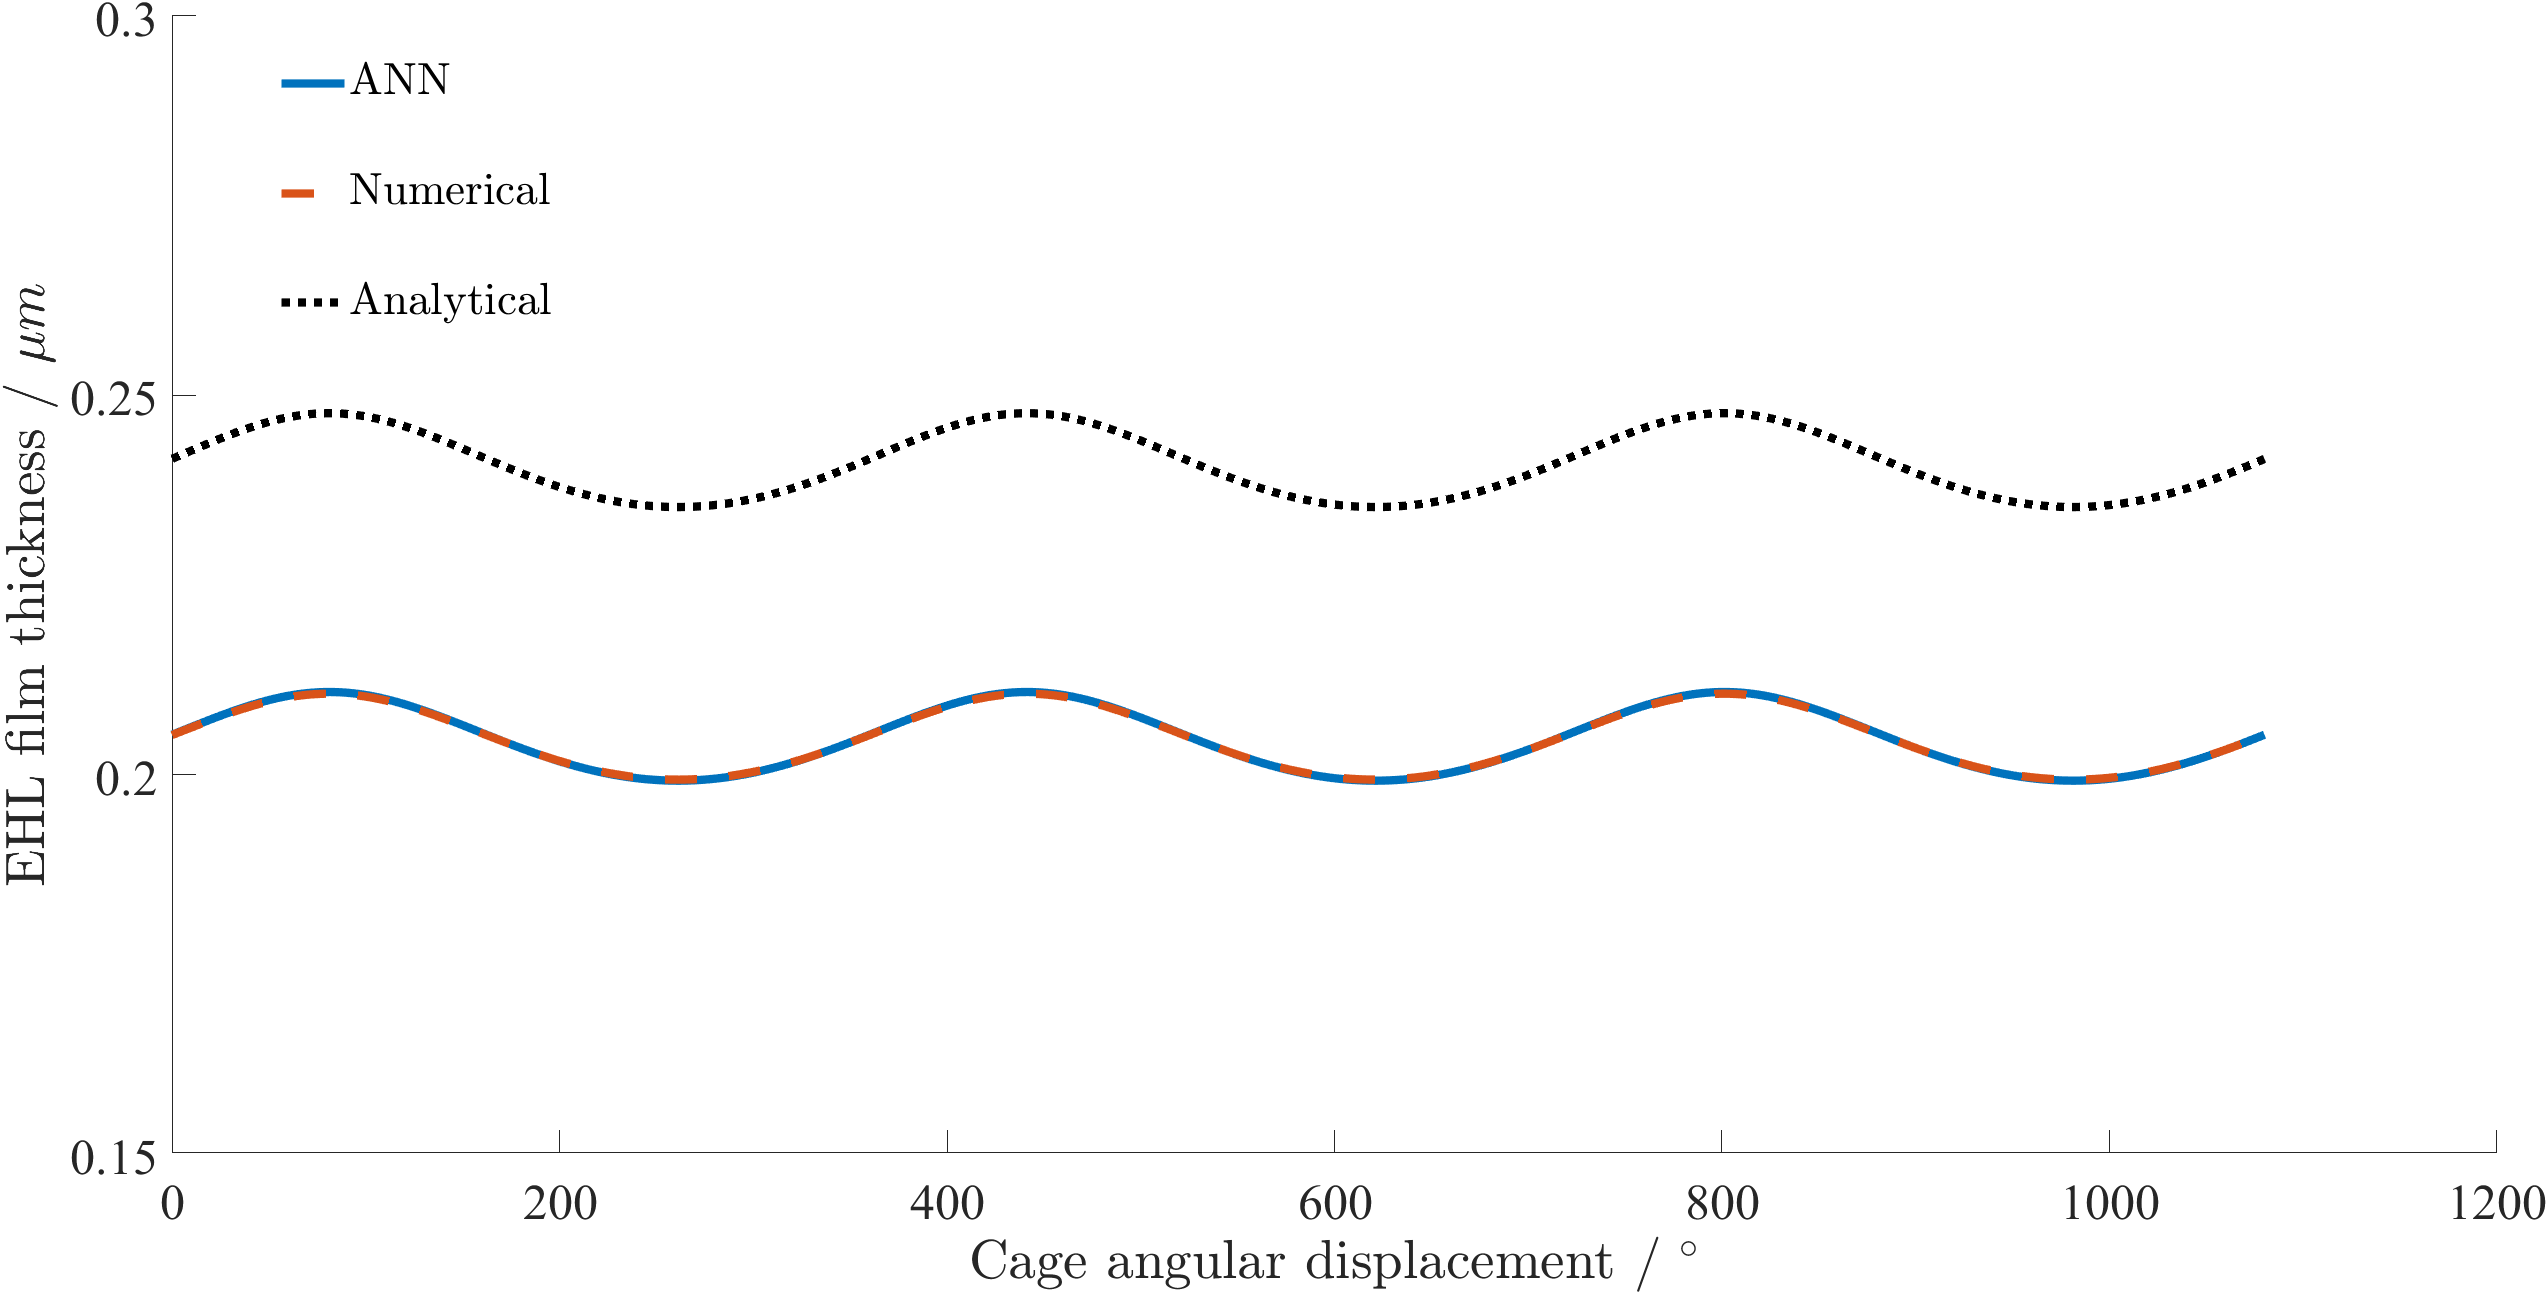
\includegraphics[width=150mm]{ANN_Explicit Film Thickness Comparisons.png}
	\caption{ANN, numerical and analytical central film thickness comparisons.}
	\label{ANN Film Thickness Comparisons}
\end{figure}
Figure 

Three different methods of obtaining the EHL film thickness were tested

\begin{tabular}{|c|c|c|}
	\hline \multirow{2}{*}{ Method } & \multicolumn{2}{|c|}{ Bearing } \\
	\cline { 2 - 3 } & Time per point & MSE \\
	\cline { 2 - 3 } & {$[\mathrm{s}]$} & {$[\mu \mathrm{m}]$} \\
	\hline Numerical & $4.87 \mathrm{E}+00$ & - \\
	\hline Analytical & $4.43 \mathrm{E}-05$ & $1.32 \mathrm{E}-3$ \\
	\hline ANN & $3.33 \mathrm{E}-03$ & $1.46 \mathrm{E}-8$ \\
	\hline
\end{tabular}




\section{Conclusions}





\section{Conclusions}
Roller bearings are only one application of these ANNs. The use cases extend far beyond roller bearings, to key components in automotive, machining and other industrial applications where interactions between contiguous surfaces exist. Film thickness is a critical parameter in the determination of NVH, friction and wear.

Full numerical solution can account for film thickness profile and pressure distribution across the contact. Futhermore, 

Echávarri et al. \cite{EchavarriOtero2014} comment on the "black box" nature of ANNs. Results from intermediate calculations are lost, which is often of interest for more in-depth analysis of contact condition; film thickness and pressure distributions and temperature for example. 

